% Full-length journal version in the IEEE Access format: every derivation, figure, table and experiment.
% Build: cd paper && make access.pdf   (class ieeeaccess.cls + access/*.png from the IEEE Access LaTeX
% template; the template's commercial fonts Formata/Giovanni fall back to standard ones).
% The sections live in sections/access_*.tex so that several people can edit them at once.
% Every number comes from tables/numbers.tex or tables/tab_*.tex (paper/make_assets.py). Never type results.
\documentclass{ieeeaccess}
\IEEEoverridecommandlockouts
\year{2026}                   % ieeeaccess.cls turns the TeX primitive \year into "set the header year";
\ExplSyntaxOn\cs_set_eq:NN\year\tex_year:D\ExplSyntaxOff   % pgf and \today need the primitive: restore it
\providecommand\xfigwd{0pt}   % the class's captions read the width that its own \Figure macro sets
\definecolor{accessblue}{cmyk}{1,0.3,0,0.2}   % PANTONE 3015 C as process colour (the class's spot colour
                                             % space is not written correctly: invisible title)
\graphicspath{{access/}{./}}
% Shared by conference.tex (IEEEtran, 6 pages) and access.tex (IEEE Access, full length).
% Every number in either paper comes from tables/numbers.tex or tables/tab_*.tex, which
% paper/make_assets.py generates from paper/data/. Do not type results by hand.
\usepackage{cite}
\usepackage{amsmath,amssymb}
\usepackage{graphicx}
\usepackage{booktabs}
\usepackage{xcolor}
\usepackage{tikz}
\usetikzlibrary{arrows.meta,positioning,fit,calc,backgrounds,shapes.geometric,decorations.pathreplacing}
\usepackage[siunitx,american]{circuitikz}
% Shared TikZ styles for the hand-drawn architecture and circuit figures (paper/figures/tikz/*.tex).
% Both papers load this file; every figure here is drawn from the RTL (rtl/*.v) and the block design
% (future_work/board/block_design.tcl) it depicts, so keep them in sync when either changes.
\definecolor{psfill}{RGB}{226,236,250}
\definecolor{plfill}{RGB}{252,236,218}
\definecolor{cryfill}{RGB}{250,214,214}
\definecolor{netfill}{RGB}{236,236,236}
\definecolor{rxfill}{RGB}{222,242,226}
\definecolor{inkc}{RGB}{40,40,40}
\tikzset{
  blk/.style={draw=inkc, rounded corners=1pt, minimum height=6mm, align=center, inner sep=2pt, font=\scriptsize, fill=white},
  cry/.style={blk, fill=cryfill},
  arm/.style={blk, fill=psfill},
  pl/.style={blk, fill=plfill},
  rx/.style={blk, fill=rxfill},
  grp/.style={draw=inkc, rounded corners=3pt, inner sep=3mm},
  arr/.style={-{Latex[length=1.5mm]}, inkc},
  darr/.style={{Latex[length=1.5mm]}-{Latex[length=1.5mm]}, inkc},
  bus/.style={-{Latex[length=1.6mm]}, line width=0.9pt, inkc},
  lbl/.style={font=\tiny, inner sep=1pt},
  ttl/.style={font=\scriptsize\bfseries, inner sep=1pt},
}

\newcommand{\TODO}[1]{\textcolor{red}{[TODO: #1]}}
% \ifextended: content only in the full-length (IEEE Access) version; the generated tables use it too
\newif\ifextended
% generated by paper/make_assets.py from paper/data -- do not edit
\newcommand{\AesGcmMs}{0.01}
\newcommand{\AllDecode}{all}
\newcommand{\BenignFalse}{0/447}
\newcommand{\BenignLatency}{82}
\newcommand{\BenignPninetyfive}{278}
\newcommand{\BenignRuns}{3}
\newcommand{\CostEfive}{31.0}
\newcommand{\CostEfour}{29.5}
\newcommand{\CostEtwo}{13.4}
\newcommand{\CryptoLutShare}{54}
\newcommand{\CyclesPerPixel}{1.64}
\newcommand{\Decoders}{Pillow, OpenCV, scikit-image, FFmpeg (MJPEG)}
\newcommand{\FbDropTtm}{3.5}
\newcommand{\FpsHD}{66}
\newcommand{\FpsVGA}{199}
\newcommand{\JigsawNeighboursMax}{1.7}
\newcommand{\JigsawOracleMax}{0.47}
\newcommand{\JigsawOracleMin}{0.41}
\newcommand{\LeakEFiveMax}{0.017}
\newcommand{\LeakEFiveMin}{-0.004}
\newcommand{\LeakEOneFourMax}{0.58}
\newcommand{\LeakEOneFourMin}{0.27}
\newcommand{\LearnEfiveEdgeMax}{0.021}
\newcommand{\LearnEpochs}{25}
\newcommand{\LearnSsimMax}{0.43}
\newcommand{\LearnTest}{400}
\newcommand{\LearnTrain}{1000}
\newcommand{\MaxExtraCycles}{5}
\newcommand{\NumAttacks}{11}
\newcommand{\NumClips}{4}
\newcommand{\NumDecoders}{4}
\newcommand{\OverheadEfiveQVGA}{12}
\newcommand{\OverheadEfiveVGA}{21}
\newcommand{\OverheadEtwoQVGA}{0.5}
\newcommand{\OverheadEtwoVGA}{0.3}
\newcommand{\PolCostB}{0.162}
\newcommand{\PolCostSave}{14}
\newcommand{\PolCostT}{0.188}
\newcommand{\PolFalse}{0/6020}
\newcommand{\PolLeakB}{0.054}
\newcommand{\PolTtmB}{1.34}
\newcommand{\PolTtmT}{0.46}
\newcommand{\PyPlainMs}{134}
\newcommand{\PySelEtwoMs}{151}
\newcommand{\RealTalkFalse}{0/125}
\newcommand{\RealTalkMit}{11/11}
\newcommand{\RealTalkTtm}{1.09}
\newcommand{\RealTrailerFalse}{0/125}
\newcommand{\RealTrailerMit}{11/11}
\newcommand{\RealTrailerTtm}{0.89}
\newcommand{\ResourceSource}{a Yosys synthesis estimate}
\newcommand{\Seeds}{10}
\newcommand{\SuiteFalse}{0/375}
\newcommand{\SuiteLatency}{97}
\newcommand{\SuiteRuns}{3}
\newcommand{\TopLutPct}{10.7}
\newcommand{\TopLuts}{5{,}681}
\newcommand{\TtmMean}{0.91}
\newcommand{\TtmSd}{0.02}
\newcommand{\TurboFps}{1047}
\newcommand{\TurboMs}{0.95}

% ---------------------------------------------------------------- notation (Section "Notation" in access.tex)
\newcommand{\xor}{\oplus}
\newcommand{\cat}{\,\|\,}
\newcommand{\Kseg}{K_{\mathrm{seg}}}
\newcommand{\Kfb}{K_{\mathrm{fb}}}
\newcommand{\Nenc}{N^{\mathrm{enc}}}
\newcommand{\Nmac}{N^{\mathrm{mac}}}
\newcommand{\Enc}{\mathcal{E}}
\newcommand{\MAC}{\mathrm{MAC}}
\newcommand{\KDF}{\mathrm{KDF}}
\newcommand{\amp}{\mathcal{A}}
\newcommand{\sz}{\mathrm{cat}}

\usepackage{amsthm}
\newtheorem{proposition}{Proposition}
\newtheorem{lemma}{Lemma}
\theoremstyle{definition}\newtheorem{definition}{Definition}
\usepackage{algorithm}
\usepackage{algpseudocode}
\usepackage[hidelinks]{hyperref}
\extendedtrue

\begin{document}
\history{Date of publication xxxx 00, 0000, date of current version xxxx 00, 0000.}
\doi{10.1109/ACCESS.2026.DOI}
\title{Playable but Private: In-Encoder Selective Encryption with Ascon-AEAD128 and Attack-Adaptive Protection for MJPEG Video on an FPGA SoC}
\author{\uppercase{Aravind R}\authorrefmark{1}, \uppercase{Suhas V J}\authorrefmark{1}, \uppercase{Rishab H R}\authorrefmark{1}, \uppercase{Samarth B N}\authorrefmark{1}, \uppercase{Vijaysurya B S}\authorrefmark{1}, and \uppercase{Chetana G}\authorrefmark{1}\,\TODO{order, IEEE membership}}
\address[1]{Department of Electronics and Communication Engineering, RV College of Engineering, Bengaluru 560059, India \TODO{e-mails}}
\tfootnote{\TODO{funding statement, or ``This work received no external funding.''} \textcolor{red}{\textbf{Draft, \today. Not for distribution.}}}
\markboth{Aravind R \headeretal: Playable but Private}{Aravind R \headeretal: Playable but Private}
\corresp{Corresponding author: \TODO{name} (e-mail: \TODO{address}).}

\begin{abstract}
Small cameras stream over networks they do not control, yet encrypting the whole stream makes it unplayable without the key and spends cipher work on every byte. We present a JPEG/MJPEG encoder for a Zynq-7020 FPGA SoC that encrypts the sign and amplitude bits of selected DCT coefficients inside the entropy coder, with a keystream from the NIST SP~800-232 standard Ascon-AEAD128. We prove that the transformation never changes a Huffman code length, so every protection level is a valid JPEG, and a 128-bit tag over the frame metadata and the coded scan rejects any modified, replayed or forged frame. The strongest level hides block positions with a keyed, per-frame permutation of restart segments that needs no frame buffer: the fabric codes and authenticates one segment per macroblock and the processor only reorders them. The design is bit-exact with a golden model in simulation and on a PYNQ-Z2 board in all six levels, adds no cycles for encryption, closes timing at \TopMhz\,MHz and, with four lanes, reaches \RtlFourLanesMpix\,Mpixel/s in cycle-accurate RTL simulation. In a benchmark of four keyless attacks on \BenchSources{} sources, four re-implemented published schemes leak \BenchPubMin--\BenchPubMax{} edge correlation while our permutation level stays at or below \BenchEfiveMax{}, also against jigsaw solvers, sign-recovery optimization and trained neural attackers. An authenticated feedback loop with a forward-secure ratchet mitigates all \NumAttacks{} modelled network attacks in \TtmMean\,s on average with no false alarms.
\end{abstract}

\begin{keywords}
selective encryption, MJPEG, Ascon, lightweight cryptography, FPGA, authenticated encryption, hardware security, video surveillance
\end{keywords}

\titlepgskip=-21pt
\maketitle

% =====================================================================================================
\section{Introduction}\label{sec:intro}
Home cameras, video doorbells and baby monitors send video over Wi-Fi and shared networks that their owners do not control. Two properties matter for such a link. \emph{Confidentiality} keeps a bystander on the network from watching the home; \emph{integrity} lets the viewer trust that what it shows was captured by the camera and was not edited, replayed or injected on the way. Encrypting the transport with TLS, SRTP~\cite{rfc3711} or a VPN provides both, but it hides the stream from every recorder, player and cloud service outside the key infrastructure, and the cipher work grows with the full bitrate of a low-power device.

Selective encryption encrypts only the parts of the compressed stream that carry most of the picture and keeps the format~\cite{massoudi2008}, so standard decoders still parse the result. For baseline JPEG, the sign and the appended amplitude bits of the quantized DCT coefficients can be encrypted without changing any Huffman code length~\cite{vandroogenbroeck2002,auer2013}. Such schemes are easy to weaken: the positions of the non-zero coefficients stay visible, so an attacker still sees the outline of the scene~\cite{massoudi2008,lin2024,hirose2024}; most use key material that does not change from frame to frame, so one known frame exposes the next; and almost none authenticate what they encrypt.

We ask how much of a secure camera link fits into the encoder hardware, and what an eavesdropper still learns. Our contributions are:
\begin{enumerate}
\item \textit{Authenticated selective encryption inside the entropy coder.} A Verilog MJPEG encoder XORs a keystream of the NIST standard Ascon-AEAD128~\cite{sp800232,ascon} onto coefficient signs and amplitudes. We prove that every code length is preserved (Lemma~\ref{lem:format}) and that the cipher never stalls the encoder (Proposition~\ref{prop:supply}); a 128-bit tag binds the scan to the protection level, session, frame counter and size.
\item \textit{A hardware form of a keyed macroblock permutation (E5).} The fabric codes one restart segment per macroblock with its own keystream and authenticates them in raster order; the ARM core sends them in a keyed order that changes with every frame. No frame buffer is needed, and the order is authenticated.
\item \textit{Parallel lanes and a measured system.} Restart segments make lanes independent; one, two and four lanes produce identical bytes. On a PYNQ-Z2 board every image is bit-exact with the golden model in every level, and the encoding clocks counted by the fabric equal the RTL simulation's to within \BdBusyVsRtlMaxPct\,\% (four lanes: \BdFourBusyMpix\,Mpixel/s at \BdFourMhz\,MHz).
\item \textit{One benchmark for all schemes.} Six protection levels and four published format-compliant schemes~\cite{vandroogenbroeck2002,kishore2015,auer2013,hirose2024} under the same keyless attacks, including puzzle solvers, sign recovery, a chosen-plaintext attack and trained networks, on \NumVideoClips{} clips and the Kodak set.
\item \textit{A closed feedback loop.} An authenticated feedback channel, a forward-secure key ratchet and an adaptive policy raise protection when the receiver reports an attack, in simulation and with the board as the camera.
\end{enumerate}
\TODO{Once the conference version is accepted: cite it here and state what this article adds (proofs, board evaluation, full benchmark, protocol analysis).}

% =====================================================================================================
\section{Related Work}\label{sec:related}
\textit{Selective encryption of JPEG.} Van Droogenbroeck and Benedett encrypted the appended bits of AC coefficients and kept the Huffman code words~\cite{vandroogenbroeck2002}; Puech and Rodrigues encrypted selected DCT coefficients with AES in OFB mode~\cite{puech2005}; Auer et al.\ permuted code-word/value pairs and toggled value bits at bitstream level at more than 25 VGA frames per second~\cite{auer2013}. Massoudi et al.\ note that visual distortion does not measure security~\cite{massoudi2008}. The idea has been carried to H.264/AVC and HEVC~\cite{boyadjis2017}.

\textit{Attacks.} Lin et al.\ recover DCT sign bits by linear programming~\cite{lin2024}. Hirose et al.\ show that the number of non-zero coefficients per block, which no field encryption hides, rebuilds contours unless the restart segments are permuted~\cite{hirose2024}; Li et al.\ recover block shuffles from one designed plaintext~\cite{li2025shuffle}; a GAN-based ciphertext-only attack recovers content from most privacy-preserving image schemes~\cite{sirichotedumrong2020}; and block permutations invite jigsaw solvers, from greedy placement~\cite{pomeranz2011} to minimum-spanning-tree assembly~\cite{gallagher2012}.

\textit{Hardware.} Kishore et al.\ added block and symbol scrambling to an FPGA JPEG encoder at 13--17\,\% more ALUTs~\cite{kishore2015}; Ba\u{g}baba and \"Ors combined an FPGA JPEG encoder with TEA encryption of DC and low AC coefficients~\cite{bagbaba2015}; Qiu et al.\ XOR raw frames with chaotic sequences on a satellite payload~\cite{qiu2025}. None authenticates frames, and their key material is fixed. Commercial JPEG cores process one sample per clock at 150--166\,MHz without cryptography~\cite{logijpge,castjpeg}. Ascon is small in hardware, about 7\,kGE for one unrolled round, and a threshold implementation costs about 3.1 times the area of the low-area core~\cite{gross2017}; Ascon-based MACs~\cite{khairallah2023} and Ascon with replay detection~\cite{kurian2025} have been built on Artix-7. Farahmand et al.\ measure cryptographic cores on a Zynq-7020 with DMA, cycle-exact timers and bit-exact comparison with software~\cite{farahmand2016}; our board evaluation follows the same principles.

\textit{Traffic analysis.} Sizes and timing of encrypted streams reveal motion~\cite{wampler2015} and which video is played~\cite{schuster2017}; traffic shaping hides activity at a large bandwidth cost~\cite{apthorpe2019}. No content encryption changes this, so we measure it separately.

We found no design that places a standardized AEAD inside a hardware JPEG encoder, keeps every level playable while authenticating each frame, hides block positions without a frame buffer, and closes the loop from the receiver back to the encoder.

% =====================================================================================================
\section{Related Work}\label{sec:related}
\subsection{Selective encryption of JPEG}
Van Droogenbroeck and Benedett encrypted the appended bits of selected AC coefficients of baseline JPEG, leaving the Huffman code words in place, so that the stream stays compliant at a constant bit rate~\cite{vandroogenbroeck2002}. Puech and Rodrigues encrypted selected DCT coefficients of medical images with AES in OFB mode~\cite{puech2005}. Auer et al.\ encrypted baseline JPEG at bitstream level, permuting Huffman code-word/value pairs and toggling value bits, with an AES-OFB generator at more than 25 VGA frames per second, preserving length and format~\cite{auer2013}. Massoudi et al.\ survey the field and note that visual distortion is subjective and does not measure security: replacement and chosen-plaintext attacks recover more than the scrambled image suggests~\cite{massoudi2008}. Selective encryption has also been extended to H.264/AVC and HEVC~\cite{boyadjis2017}.

\subsection{Attacks on format-compliant encryption}
Lin et al.\ show that DCT sign bits can be recovered by linear programming~\cite{lin2024}, which bounds what sign-only encryption can promise. Hirose et al.\ analyse bitstream-level JPEG encryption that shuffles blocks delimited by restart markers; the number of non-zero coefficients per block, which no field encryption hides, recovers contours unless the segments are permuted, and partly again when the restart interval is large~\cite{hirose2024}. Our strongest level uses the same mechanism with a keyed, per-frame permutation. Li et al.\ recover block-shuffled JPEG with a designed plaintext that reveals the permutation through its per-block non-zero counts, which then inverts any image shuffled with the same permutation~\cite{li2025shuffle}. Learned attackers are a threat beyond hand-made ones: Sirichotedumrong and Kiya find that a GAN-based ciphertext-only attack recovers visual content from most image-protection schemes designed for privacy-preserving deep learning~\cite{sirichotedumrong2020}. Block permutations also invite jigsaw solvers, from greedy placement~\cite{pomeranz2011} to minimum-spanning-tree assembly with gradient compatibility~\cite{gallagher2012}.

\subsection{Hardware JPEG encoders with encryption}
Kishore et al.\ added PN-sequence block and symbol scrambling to an FPGA JPEG encoder for 256$\times$256 grey images on Stratix~II and~IV; they describe the extra hardware as about 1\,\%, while their tables show 13--17\,\% more ALUTs, twice the memory bits and 9--10\,\% fewer frames per second with it~\cite{kishore2015}. Ba\u{g}baba and \"Ors combined an FPGA JPEG encoder with TEA encryption of the DC coefficients, or of the DC and first five AC coefficients, of every block~\cite{bagbaba2015}. Neither authenticates the frames, and both use key material that does not change from frame to frame. Qiu et al.\ XOR raw video frames with two one-dimensional chaotic sequences in real time on a satellite payload (a Raspberry Pi~4B) and also implement the maps on an FPGA; their output is neither a compressed stream nor authenticated~\cite{qiu2025}. Commercial JPEG encoder cores process one sample per clock at 150--166\,MHz without cryptography~\cite{logijpge,castjpeg}.

\subsection{Lightweight authenticated encryption in hardware}
Ascon, now standardized by NIST in SP~800-232~\cite{sp800232,ascon}, is small and fast in hardware: a core with one unrolled round takes about 7\,kGE, and a threshold implementation against power analysis costs about 3.1 times the area of the unprotected low-area core~\cite{gross2017}. Khairallah and Yadhunathan compare FPGA message-authentication codes built on the Ascon permutation on Artix-7~\cite{khairallah2023}. Gladis Kurian and Chen implement Ascon on an Artix-7 with replay detection through a Bloom filter in block RAM, which has no false negatives but a small false-positive rate (0.17\,\% measured)~\cite{kurian2025}.

\subsection{Traffic analysis of encrypted video}
Sizes and timing of encrypted streams reveal motion~\cite{wampler2015} and which video is played~\cite{schuster2017}; traffic shaping hides IoT activity at up to $18\times$ the bandwidth for a camera~\cite{apthorpe2019}. No encryption of content changes this, so we measure it separately (Section~\ref{sec:discussion}).

\subsection{How hardware designs in this field are evaluated}\label{sec:evalpractice}
Table~\ref{tab:evalpractice} summarizes what the hardware papers above report and how. Most stop at synthesis or place and route: Kishore et al.\ give post-synthesis resources and compute the maximum frame rate as the inverse of the coding time of one frame at the synthesized clock~\cite{kishore2015}; Ba\u{g}baba and \"Ors target a Virtex-6 ML605 kit and evaluate the encryption by PSNR and RMSE~\cite{bagbaba2015}; Khairallah and Yadhunathan report Vivado synthesis results including power~\cite{khairallah2023}; Gladis Kurian and Chen implement their design on an Arty A7-100T, show replay detection on the board with LED indicators and report on-chip power split into static and dynamic parts~\cite{kurian2025}. The most complete measurement methodology we found is the Zynq-7020 testbed of Farahmand et al.\ for cryptographic cores: an AXI DMA streams data between DDR and the core, an AXI timer measures hardware and software time to one clock cycle, every hardware output is compared with software, and the clock is raised by binary search to the highest frequency that still gives correct results~\cite{farahmand2016}. We follow the same principles: bit-exact comparison with a reference for every frame, cycle-accurate throughput, post-route timing and power with simulated switching activity, and a board protocol with the same DMA structure (Section~\ref{sec:board}).

\begin{table*}[t]
\caption{How related hardware designs were evaluated (from each source).}
\label{tab:evalpractice}
\centering\small\setlength{\tabcolsep}{4pt}
\resizebox{\textwidth}{!}{%
\begin{tabular}{lllll}
\toprule
Work & Platform & Area / timing & Throughput & Correctness, power \\
\midrule
Kishore~\cite{kishore2015} & Stratix II/IV & synthesis & computed from clock & PSNR; no power \\
Ba\u{g}baba~\cite{bagbaba2015} & Virtex-6 ML605 & synthesis & -- & PSNR, RMSE; no power \\
Khairallah~\cite{khairallah2023} & Artix-7 & Vivado synthesis & computed & Vivado power \\
Kurian~\cite{kurian2025} & Arty A7-100T board & Vivado & latency in simulation & LEDs on board; on-chip power \\
Farahmand~\cite{farahmand2016} & ZedBoard (Zynq-7020) & place and route & AXI timer, DMA & vs.\ software; max.\ frequency search \\
\midrule
Ours & PYNQ-Z2 (Zynq-7020) & post-route, OOC + system & cycle-accurate RTL & bit-exact vs.\ model in simulation and on the board; SAIF power; board power \TODO{A4} \\
\bottomrule
\end{tabular}}
\end{table*}

\subsection{Weaknesses of prior designs and how we address them}\label{sec:weak}
Table~\ref{tab:weak} collects, from the sources above, the weaknesses that recur in format-compliant and hardware video encryption, and the part of this work that answers each. Every answer is evaluated in the sections named in the last column; none is claimed beyond what is measured there.

\begin{table*}[t]
\caption{Recurring weaknesses of prior work (from each source) and where this work addresses them.}
\label{tab:weak}
\centering\small\setlength{\tabcolsep}{4pt}
\begin{tabular}{p{0.30\textwidth}p{0.17\textwidth}p{0.33\textwidth}p{0.11\textwidth}}
\toprule
Weakness & Seen in & This work & Where \\
\midrule
No authentication: a tampered, replayed or downgraded frame is displayed & \cite{kishore2015,bagbaba2015,qiu2025} & per-frame Ascon tag over metadata and scan, replay window, authenticated level & Sec.~\ref{sec:tag}, \ref{sec:feedback} \\
Key material that does not change per frame: one known frame breaks the rest & \cite{vandroogenbroeck2002,kishore2015,hirose2024,li2025shuffle} & keystream and E5 permutation drawn anew from (session, frame counter) & Sec.~\ref{sec:nonce}, \ref{sec:bench} \\
Field encryption leaves outlines (non-zero counts per block) & \cite{hirose2024} & E5 permutes every MCU, keyed per frame, without a frame buffer & Sec.~\ref{sec:e5}, \ref{sec:leakage} \\
Visual distortion (PSNR) used as the security measure & \cite{bagbaba2015,kishore2015,massoudi2008} & the same hand-made and learned attacks against every scheme (SVE-Bench) & Sec.~\ref{sec:bench} \\
Grey 256$\times$256 images, or a few test images & \cite{kishore2015} & colour 4:2:0 video: open films and private clips & Sec.~\ref{sec:security} \\
Throughput computed from the synthesized clock & \cite{kishore2015,khairallah2023} & cycle-accurate RTL, post-route timing, bit-exact on the board & Sec.~\ref{sec:hwresults} \\
Probabilistic replay detection (Bloom filter false positives) & \cite{kurian2025} & a sliding 64-frame window with no false positives & Sec.~\ref{sec:feedback} \\
Output not a compressed, playable stream & \cite{qiu2025} & every level is baseline JPEG (Lemma~\ref{lem:format}) & Sec.~\ref{sec:selenc} \\
\bottomrule
\end{tabular}
\end{table*}

\subsection{Gap}
We found no design that (i)~places a standardized lightweight AEAD inside a hardware JPEG encoder at the entropy-coding stage, (ii)~keeps every protection level playable while authenticating each frame together with its metadata, (iii)~hides block positions in hardware without a frame buffer, and (iv)~closes the loop from the receiver back to the encoder so that the protection level follows observed attacks. We also could not find an evaluation that scores published format-compliant schemes and new ones under the same attacks, including learned attackers, on real video.

% =====================================================================================================
\section{Background and Notation}\label{sec:background}
Table~\ref{tab:notation} lists the symbols used in the rest of the paper. All arithmetic of this section is the bit-exact contract between the golden model and the RTL: the hardware computes exactly these integer formulas, and the tests compare every intermediate value.

\begin{table}[t]
\caption{Notation.}
\label{tab:notation}
\centering\small\setlength{\tabcolsep}{3pt}
\resizebox{\columnwidth}{!}{%
\begin{tabular}{ll}
\toprule
Symbol & Meaning \\
\midrule
$W, H$ & frame width and height (multiples of 16) \\
$M = WH/256$ & number of 16$\times$16 macroblocks (MCUs) \\
$v$, $s$, $\amp(v)$ & quantized coefficient, its size category, its appended field \\
$t$, $\sigma$, $e$ & frame counter (63 bits), session identifier (64 bits), key epoch \\
$N(\sigma, t, b)$ & 128-bit nonce, $b \in \{0,1\}$ selects keystream or tag \\
$K_{\mathrm{m}}, K_e, \Kfb$ & master key, video key of epoch $e$, feedback key \\
$\Kseg, K_\pi$ & per-frame segment key, E5 permutation key \\
$Z_s$ & keystream of restart segment $s$ \\
$T_t$, $P_t$ & tag of frame $t$, its 26-byte authenticated prefix \\
$\pi_t$ & E5 permutation of the $M$ segments of frame $t$ \\
$L$, $c_L$, $\Theta_L$ & number of lanes, cycles per pixel, throughput \\
$\xor$, $\cat$, $\ggg$ & XOR, concatenation, rotation to the right \\
\bottomrule
\end{tabular}}
\end{table}

\subsection{Baseline JPEG}
\textit{Colour and sampling.} Each pixel $(R, G, B)$ is converted with 8-bit fixed-point coefficients and clamped to $[0, 255]$:
\begin{equation}
\begin{aligned}
Y  &= \lfloor (77R + 150G + 29B + 128) / 2^8 \rfloor,\\
C_b &= \lfloor (-43R - 85G + 128B + 32896) / 2^8 \rfloor,\\
C_r &= \lfloor (128R - 107G - 21B + 32896) / 2^8 \rfloor,
\end{aligned}
\label{eq:ycc}
\end{equation}
and every 2$\times$2 group of chroma samples $a, b, c, d$ is averaged as $\lfloor (a + b + c + d + 2)/4 \rfloor$ (4:2:0). A 16$\times$16 macroblock (MCU) therefore yields six 8$\times$8 blocks, four of luma and one of each chroma component, i.e.\ 384 samples for 256 pixels, or 1.5 samples per pixel.

\textit{Transform.} The two-dimensional DCT of a block $X$ of level-shifted samples is
\begin{equation}
F(u, v) = \tfrac{1}{4} c(u) c(v) \sum_{y=0}^{7} \sum_{x=0}^{7} X(y, x)\, \phi_v(x)\, \phi_u(y)
\label{eq:dctexact}
\end{equation}
with $\phi_k(x) = \cos\frac{(2x+1)k\pi}{16}$, $c(0) = 1/\sqrt2$ and $c(k) = 1$ otherwise. The hardware uses the separable integer form with the 13-bit matrix $C(u, x) = \operatorname{round}\bigl(2^{12} c(u) \phi_u(x)\bigr)$ and two rounding passes,
\begin{equation}
\begin{aligned}
G(y, v) &= \bigl\lfloor \bigl(\textstyle\sum_{x} C(v, x)\,(X(y, x) {-} 128) + 2^{10}\bigr) / 2^{11} \bigr\rfloor,\\
F(u, v) &= \bigl\lfloor \bigl(\textstyle\sum_{y} C(u, y)\,G(y, v) + 2^{14}\bigr) / 2^{15} \bigr\rfloor,
\end{aligned}
\label{eq:dct}
\end{equation}
whose scale is $2^{13} \cdot 2^{13} / 2^{26} = 1$, so $F$ approximates the exact DCT; the first pass keeps two fractional bits, which keeps the result within one unit of the exact transform.

\textit{Quantization.} Division by the table entry $Q(u, v)$ is replaced by a 17-bit reciprocal $R(u, v) = \operatorname{round}(2^{16}/Q(u,v))$,
\begin{equation}
q = \operatorname{sgn}(F) \bigl\lfloor (|F| R + 2^{15}) / 2^{16} \bigr\rfloor,
\label{eq:quant}
\end{equation}
clamped to $[-1024, 1023]$ for DC and $[-1023, 1023]$ for AC. With $R = 2^{16}/Q + \delta$, $|\delta| \le \tfrac12$, the product deviates from $|F|/Q$ by $|F|\,|\delta|/2^{16} \le 2^{11}/2^{17} = 2^{-6}$, so~\eqref{eq:quant} equals the rounded quotient except when $|F|/Q$ lies within $2^{-6}$ of a half-integer. One DSP slice per lane replaces a divider.

\textit{Entropy coding.} The 64 coefficients are read in zig-zag order. The DC coefficient is coded as the difference $d = q_0 - q_0'$ to the previous block of the same component; each non-zero AC coefficient as a pair (run of preceding zeros, size category) followed by an appended field. For $v \ne 0$ the size category is
\begin{equation}
s(v) = \lfloor \log_2 |v| \rfloor + 1, \qquad 2^{s-1} \le |v| \le 2^s - 1,
\label{eq:size}
\end{equation}
($s \le 11$ for DC differences, $s \le 10$ for AC), and the appended field is the $s$-bit one's-complement code
\begin{equation}
\amp(v) = \begin{cases} v, & v > 0,\\ v + 2^s - 1, & v < 0. \end{cases}
\label{eq:amp}
\end{equation}
The pair goes into a Huffman code (we use the tables of Annex~K of T.81~\cite{t81,wallace1992}); a run of 16 zeros is the symbol ZRL and the rest of a block after its last non-zero coefficient is EOB. Two properties follow and our design rests on both. First, the appended field can be changed without changing the Huffman code or the stream length, as long as $s$ is kept. Second, the Huffman symbols, and with them the run lengths and size categories of every non-zero coefficient, stay visible to anyone: they carry the outline of the picture.

\textit{Restart markers.} A restart marker RST$_m$ ($\mathrm{0xFFD0} + m$, $m = 0 \ldots 7$ cyclically) ends a restart segment: the bit stream is padded to a byte with 1-bits, all DC predictors are reset to zero, and the next segment can be decoded without any knowledge of the previous one~\cite{t81}. A DRI segment in the header gives the number of MCUs per segment. Inside segments, every byte 0xFF is followed by a stuffed 0x00, so a marker cannot occur in coded data. Restart segments make both the parallel lanes (Section~\ref{sec:lanes}) and the block permutation of E5 (Section~\ref{sec:e5}) possible.

\subsection{Ascon-AEAD128}\label{sec:ascon}
Ascon~\cite{ascon}, standardized by NIST in SP~800-232~\cite{sp800232}, is built on a 320-bit permutation applied to a state $S = x_0 \cat x_1 \cat x_2 \cat x_3 \cat x_4$ of five 64-bit words. One round is $p = p_L \circ p_S \circ p_C$:
\begin{itemize}
\item constant addition $p_C$: $x_2 \leftarrow x_2 \xor c_i$ with $c_i = 16(15 - i) + i$ for round $i$ (12 rounds: $i = 0 \ldots 11$; 8 rounds: $i = 4 \ldots 11$);
\item substitution $p_S$: a 5-bit S-box applied to the 64 bit slices $(x_0[j], \ldots, x_4[j])$ in parallel. In bitsliced form, with $a_0 = x_0 \xor x_4$, $a_4 = x_4 \xor x_3$, $a_2 = x_2 \xor x_1$ and $(t_0, \ldots, t_4) = (a_0, x_1, a_2, x_3, a_4)$,
\begin{equation}
b_i = t_i \xor (\neg t_{i+1} \wedge t_{i+2}) \quad (\text{indices mod } 5),
\label{eq:chi}
\end{equation}
followed by $x_0' = b_0 \xor b_4$, $x_1' = b_1 \xor b_0$, $x_2' = \neg b_2$, $x_3' = b_3 \xor b_2$, $x_4' = b_4$;
\item linear layer $p_L$: $x_i \leftarrow \Sigma_i(x_i) = x_i \xor (x_i \ggg r_i) \xor (x_i \ggg r_i')$ with $(r_i, r_i') = (19, 28), (61, 39), (1, 6), (10, 17), (7, 41)$.
\end{itemize}
Ascon-AEAD128 takes a 128-bit key $K$ and nonce $N$. It initializes $S \leftarrow p^{12}(\mathit{IV} \cat K \cat N) \xor (0^{192} \cat K)$; absorbs the associated data in 128-bit blocks, each XORed into $x_0 \cat x_1$ and followed by $p^8$; flips a domain-separation bit in $x_4$; encrypts each 128-bit plaintext block $P_i$ as $C_i = P_i \xor (x_0 \cat x_1)$, sets $x_0 \cat x_1 \leftarrow C_i$ and applies $p^8$; and finalizes with $S \leftarrow p^{12}(S \xor (0^{128} \cat K \cat 0^{64}))$ and the tag $T = (x_3 \cat x_4) \xor K$. Padding appends a single 1 and zeros to the last partial block. Bytes are loaded little-endian. The standard claims 128-bit security for confidentiality and integrity in the nonce-respecting setting and requires a new key when its data or decryption-failure limits are reached~\cite{sp800232}.

We use the construction in two ways. As a \emph{keystream generator}: for an all-zero message the ciphertext blocks are the rate words $x_0 \cat x_1$ after each $p^8$, i.e.\ a stream of pseudorandom bits under $(K, N)$. As a \emph{MAC}: the tag of an empty message with the data to authenticate as associated data. Both need the same core; one round per clock cycle gives 128 keystream bits every nine cycles (one cycle to absorb, eight rounds).

\subsection{Leakage and image-encryption metrics}\label{sec:metrics}
Let $I$ be the original luma and $\hat I$ a picture an attacker reconstructs. \emph{Edge correlation}, our main measure of outline leakage, is the Pearson correlation between Sobel gradient magnitudes,
\begin{equation}
\rho_E = \frac{\operatorname{cov}\bigl(|\nabla I|, |\nabla \hat I|\bigr)}{\sigma_{|\nabla I|}\,\sigma_{|\nabla \hat I|}},
\label{eq:edge}
\end{equation}
computed over all pixels; $\rho_E = 0$ means no outline, and it is insensitive to brightness and contrast, which a learned attacker recovers from global statistics. We also report SSIM~\cite{ssim}. For comparability with image-encryption papers we compute, between two pictures $C_1$, $C_2$ of $N$ pixels, $\mathrm{NPCR} = \frac{100}{N} \sum_{i} [C_1(i) \ne C_2(i)]$ and $\mathrm{UACI} = \frac{100}{N} \sum_{i} |C_1(i) - C_2(i)| / 255$, the histogram entropy $-\sum_k p_k \log_2 p_k$ and the correlation of adjacent pixels. These metrics were designed for ciphers that turn the whole image into noise; a format-compliant scheme keeps the stream decodable by design, so we read them together with~\eqref{eq:edge}.

% =====================================================================================================
\section{Threat Model and Security Goals}\label{sec:threat}
\textit{System.} A camera node (the PYNQ-Z2 board) encodes video and sends one JPEG per frame over UDP to a viewer; the viewer returns heartbeats and alerts over a feedback channel. Both ends hold a 128-bit master key $K_{\mathrm{m}}$ provisioned at installation. As in SRTP, whose key management is a separate protocol~\cite{rfc3711}, and in every scheme we compare with~\cite{vandroogenbroeck2002,kishore2015,auer2013,hirose2024,bagbaba2015}, key distribution is out of scope; a standard key exchange on the ARM core at session start is the natural extension (Section~\ref{sec:discussion}).

\textit{Adversary.} The attacker sits on the network path. It observes all traffic and may modify, drop, delay, replay, reorder or inject both video and feedback datagrams; it does not hold the keys. It knows the design, the code and the format, may know some frames in clear (known plaintext), may choose content that the camera films (chosen plaintext), and may train neural networks on any amount of public video. A passive eavesdropper sends nothing, so it cannot be detected; against it only the configured minimum protection level helps. Physical and side-channel attacks on the device are out of scope; a deployment that needs them can use a threshold implementation of Ascon, which Gro{\ss} et al.\ built at about 3.1 times the area of their unprotected low-area core~\cite{gross2017}.

\textit{Assets and goals.}
\begin{itemize}
\item[G1] \emph{Content confidentiality:} a keyless observer should not recover the shape of the scene. Format compliance means that the frame size, the image dimensions, the protection level and coarse statistics are public by design; we measure what else leaks (Section~\ref{sec:security}) and what the public parts reveal (Section~\ref{sec:discussion}).
\item[G2] \emph{Integrity and authenticity} of every frame together with its metadata (level, session, counter, size): any change must be rejected.
\item[G3] \emph{Freshness:} no replayed or re-ordered old frame is shown as current.
\item[G4] \emph{Availability signal:} the viewer must learn that the camera is alive, and the camera that the viewer receives; silence must be treated as an attack.
\item[G5] \emph{Forward secrecy across epochs:} a video key captured later does not decrypt earlier epochs.
\end{itemize}
G2--G5 are enforced cryptographically (Section~\ref{sec:design}); G1 is a property of the protection level, which we measure empirically against the strongest attackers we could build. The receiver accepts a frame only if its tag verifies, so a wrong key, a modified frame or a forged frame is rejected rather than shown as noise; a viewer without the key can still play the stream, which is the point of format compliance.

% =====================================================================================================
\section{Cryptographic Design}\label{sec:design}
\begin{figure*}[t]
\centering
\resizebox{0.95\textwidth}{!}{% System architecture: PYNQ-Z2 (PL + PS), network with attacker, receiver, feedback loop.
% Drawn from: future_work/board/block_design.tcl (DMA, HP0, GP0, IRQ), future_work/board/pynq_driver.py
% and board_sender.py (ARM side), link/receiver.py and link/feedback.py (receiver, feedback).
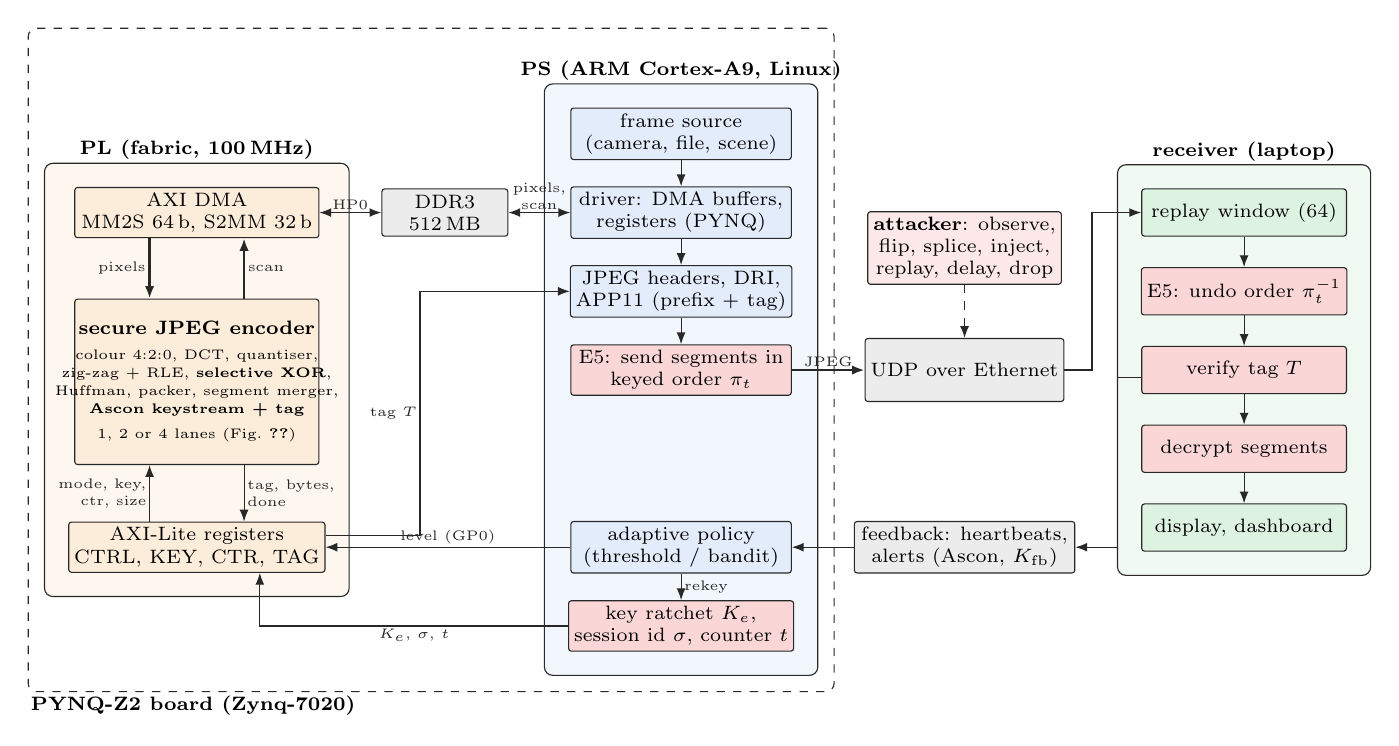
\begin{tikzpicture}[x=1cm, y=1cm]
% ---------------- PL (fabric)
\node[pl, minimum width=31mm] (dma) at (1.6,-0.6) {AXI DMA\\MM2S 64\,b, S2MM 32\,b};
\node[pl, minimum width=31mm, minimum height=21mm] (enc) at (1.6,-2.75) {};
\node[align=center, font=\scriptsize] at (enc.center) {\textbf{secure JPEG encoder}\\[1pt]
  \tiny colour 4:2:0, DCT, quantiser,\\[-1.5pt]\tiny zig-zag + RLE, \textbf{selective XOR},\\[-1.5pt]
  \tiny Huffman, packer, segment merger,\\[-1.5pt]\tiny \textbf{Ascon keystream + tag}\\[1pt]\tiny 1, 2 or 4 lanes (Fig.~\ref{fig:pl})};
\node[pl, minimum width=31mm] (regs) at (1.6,-4.85) {AXI-Lite registers\\CTRL, KEY, CTR, TAG};
\draw[bus] ([xshift=-6mm]dma.south) -- node[lbl, left]{pixels} ([xshift=-6mm]enc.north);
\draw[bus] ([xshift=6mm]enc.north) -- node[lbl, right]{scan} ([xshift=6mm]dma.south);
\draw[arr] ([xshift=-6mm]regs.north) -- node[lbl, left, align=right]{mode, key,\\ctr, size} ([xshift=-6mm]enc.south);
\draw[arr] ([xshift=6mm]enc.south) -- node[lbl, right, align=left]{tag, bytes,\\done} ([xshift=6mm]regs.north);
\begin{scope}[on background layer]
\node[grp, fill=plfill!40, fit=(dma)(enc)(regs), label={[ttl]north:PL (fabric, 100\,MHz)}] (plg) {};
\end{scope}
% ---------------- DDR
\node[blk, fill=netfill, minimum width=16mm] (ddr) at (4.75,-0.6) {DDR3\\512\,MB};
% ---------------- PS (ARM)
\node[arm, minimum width=28mm] (src) at (7.75,0.4)  {frame source\\(camera, file, scene)};
\node[arm, minimum width=28mm] (drv) at (7.75,-0.6) {driver: DMA buffers,\\registers (PYNQ)};
\node[arm, minimum width=28mm] (hdr) at (7.75,-1.6) {JPEG headers, DRI,\\APP11 (prefix + tag)};
\node[cry, minimum width=28mm] (perm) at (7.75,-2.6) {E5: send segments in\\keyed order $\pi_t$};
\node[arm, minimum width=28mm] (pol) at (7.75,-4.85) {adaptive policy\\(threshold / bandit)};
\node[cry, minimum width=28mm] (kr) at (7.75,-5.85) {key ratchet $K_e$,\\session id $\sigma$, counter $t$};
\begin{scope}[on background layer]
\node[grp, fill=psfill!45, fit=(src)(kr), label={[ttl]north:PS (ARM Cortex-A9, Linux)}] (ps) {};
\coordinate (pstop) at ([yshift=5mm]ps.north);
\node[grp, dashed, fit=(plg)(ps)(ddr)(pstop), inner sep=2mm, label={[ttl, anchor=north west]south west:PYNQ-Z2 board (Zynq-7020)}] (board) {};
\end{scope}
\draw[arr] (src) -- (drv); \draw[arr] (drv) -- (hdr); \draw[arr] (hdr) -- (perm);
\draw[darr] (drv.west) -- node[lbl, above, align=center]{pixels,\\scan} (ddr.east);
\draw[darr] (ddr.west) -- node[lbl, above]{HP0} (dma.east);
\draw[arr] (pol.west) -- node[lbl, above]{level (GP0)} (regs.east);
\draw[arr] (kr.west) -| node[lbl, pos=0.25, below]{$K_e$, $\sigma$, $t$} ([xshift=8mm]regs.south);
\draw[arr] ([yshift=1.5mm]regs.east) -- ++(1.2,0) |- node[lbl, pos=0.25, left]{tag $T$} (hdr.west);
\draw[arr] (pol.south) -- node[lbl, right]{rekey} (kr.north);
% ---------------- network
\node[blk, fill=netfill, minimum width=24mm, minimum height=8mm] (net) at (11.35,-2.6) {UDP over Ethernet};
\node[blk, fill=cryfill!55, minimum width=24mm, align=center] (atk) at (11.35,-1.05) {\textbf{attacker}: observe,\\flip, splice, inject,\\replay, delay, drop};
\draw[arr, dashed] (atk) -- (net);
\node[blk, fill=netfill, minimum width=28mm, align=center] (fb) at (11.35,-4.85) {feedback: heartbeats,\\alerts (Ascon, $K_{\mathrm{fb}}$)};
\draw[bus] (perm.east) -- node[lbl, above]{JPEG} (net.west);
\draw[arr] (fb.west) -- (pol.east);
% ---------------- receiver
\node[rx, minimum width=26mm] (rw) at (14.9,-0.6) {replay window (64)};
\node[cry, minimum width=26mm] (unp) at (14.9,-1.6) {E5: undo order $\pi_t^{-1}$};
\node[cry, minimum width=26mm] (tag) at (14.9,-2.6) {verify tag $T$};
\node[cry, minimum width=26mm] (dec) at (14.9,-3.6) {decrypt segments};
\node[rx, minimum width=26mm] (show) at (14.9,-4.6) {display, dashboard};
\begin{scope}[on background layer]
\node[grp, fill=rxfill!45, fit=(rw)(show), label={[ttl]north:receiver (laptop)}] (rxg) {};
\end{scope}
\draw[arr] (rw) -- (unp); \draw[arr] (unp) -- (tag); \draw[arr] (tag) -- (dec); \draw[arr] (dec) -- (show);
\draw[arr] (net.east) -- ++(0.35,0) |- (rw.west);
\draw[arr] (tag.west) ++(0,-0.1) -- ++(-0.3,0) |- (fb.east);
\end{tikzpicture}
}
\caption{System architecture. The programmable logic (PL) encodes, encrypts and tags every frame; the ARM core (PS) moves pixels and scan through DDR with an AXI DMA, adds the JPEG headers and the APP11 segment with the tag, sends E5 segments in the keyed order, and runs the key ratchet and the adaptive policy. The receiver undoes the order, verifies the tag, decrypts, and reports back over an authenticated feedback channel. Shaded red: cryptographic operations.}
\label{fig:system}
\end{figure*}

\subsection{Overview}
Fig.~\ref{fig:system} shows the system. The ARM core of the Zynq places a frame in DDR, writes the per-frame registers (level, counter, size) and starts the DMA; the fabric reads the pixels, codes them into a JPEG scan in which the selected coefficient fields are encrypted, computes the frame tag over the metadata and the scan, and writes the scan back. The ARM core reads the tag, wraps the scan in standard JPEG headers and an application segment (APP11) that carries the metadata and the tag, reorders the segments if the level is E5, and sends the frame in UDP datagrams. All per-byte cryptographic work happens in the fabric; the ARM touches each output byte once.

\subsection{Keys, nonces and their uniqueness}\label{sec:nonce}
\begin{figure*}[t]
\centering
\resizebox{0.78\textwidth}{!}{% Key and nonce hierarchy (link/keys.py, model/ascon.py :: make_nonce, model/hw.py :: shuffle_key,
% rtl/kseg_unit.v). KDF(K, label, c) = Ascon-AEAD128 tag under K, nonce (sigma = 0, c, purpose 1), AD = label.
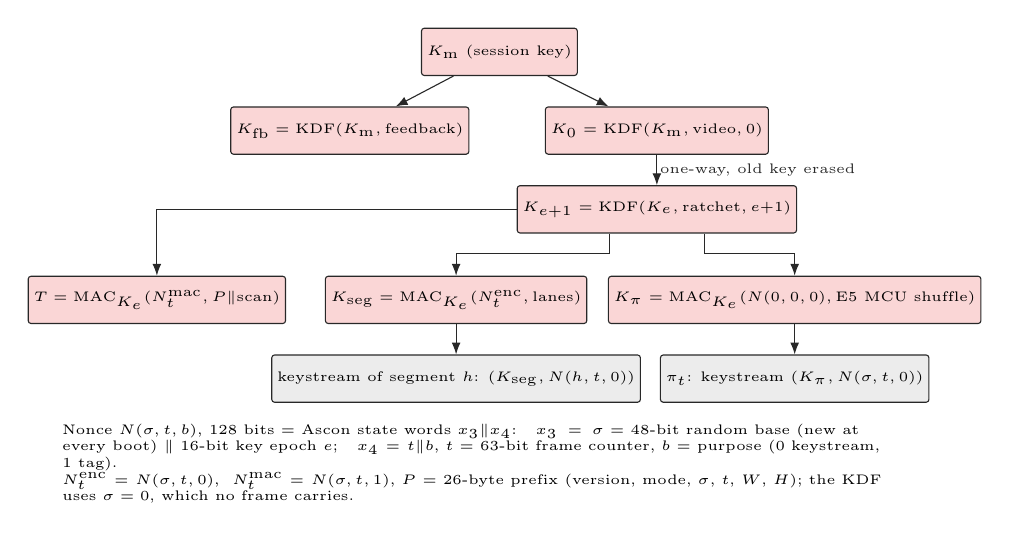
\begin{tikzpicture}[x=1cm, y=1cm, k/.style={cry, font=\tiny, minimum height=6mm}, n/.style={blk, font=\tiny, fill=netfill, minimum height=6mm}]
\node[k] (m) at (0,0) {$K_{\mathrm{m}}$ (session key)};
\node[k] (fb) at (-1.9,-1.0) {$K_{\mathrm{fb}} = \mathrm{KDF}(K_{\mathrm{m}}, \text{feedback})$};
\node[k] (v0) at (2.0,-1.0) {$K_0 = \mathrm{KDF}(K_{\mathrm{m}}, \text{video}, 0)$};
\node[k] (ve) at (2.0,-2.0) {$K_{e+1} = \mathrm{KDF}(K_e, \text{ratchet}, e{+}1)$};
\draw[arr] (m) -- (fb); \draw[arr] (m) -- (v0); \draw[arr] (v0) -- node[lbl, right]{one-way, old key erased} (ve);
\node[k] (ks) at (-0.55,-3.15) {$K_{\mathrm{seg}} = \mathrm{MAC}_{K_e}(N^{\mathrm{enc}}_t, \text{lanes})$};
\node[k] (kp) at (3.75,-3.15) {$K_\pi = \mathrm{MAC}_{K_e}(N(0,0,0), \text{E5 MCU shuffle})$};
\draw[arr] (ve.south) ++(-0.6,0) |- ++(0,-0.25) -| (ks.north);
\draw[arr] (ve.south) ++(0.6,0) |- ++(0,-0.25) -| (kp.north);
\node[k] (tg) at (-4.35,-3.15) {$T = \mathrm{MAC}_{K_e}(N^{\mathrm{mac}}_t, P \| \mathrm{scan})$};
\draw[arr] (ve.west) -| (tg.north);
\node[n] (z) at (-0.55,-4.15) {keystream of segment $h$: $(K_{\mathrm{seg}}, N(h, t, 0))$};
\node[n] (p) at (3.75,-4.15) {$\pi_t$: keystream $(K_\pi, N(\sigma, t, 0))$};
\draw[arr] (ks) -- (z); \draw[arr] (kp) -- (p);
\node[font=\tiny, align=left, anchor=north, text width=105mm] at (-0.3,-4.6) {Nonce $N(\sigma, t, b)$, 128 bits = Ascon state words $x_3 \| x_4$:\quad
$x_3 = \sigma$ = 48-bit random base (new at every boot) $\|$ 16-bit key epoch $e$;\quad
$x_4 = t \| b$, $t$ = 63-bit frame counter, $b$ = purpose (0 keystream, 1 tag).\\
$N^{\mathrm{enc}}_t = N(\sigma, t, 0)$,\ \ $N^{\mathrm{mac}}_t = N(\sigma, t, 1)$, $P$ = 26-byte prefix (version, mode, $\sigma$, $t$, $W$, $H$); the KDF uses $\sigma = 0$, which no frame carries.};
\end{tikzpicture}
}
\caption{Key and nonce hierarchy. One pre-shared master key yields the feedback key and the epoch-0 video key; a one-way ratchet yields every later epoch. Per frame, the video key derives the segment key (keystream) and the E5 permutation key and authenticates the frame.}
\label{fig:keys}
\end{figure*}
All keys derive from $K_{\mathrm{m}}$ with one primitive, the Ascon tag used as a pseudorandom function (Fig.~\ref{fig:keys}):
\begin{equation}
\KDF(K, \ell, c) = \MAC_K\bigl(N(0, c, 1), \ell\bigr),
\label{eq:kdf}
\end{equation}
the tag of an empty message with label $\ell$ as associated data, under a nonce with session identifier $0$, which no frame carries. The feedback key is $\Kfb = \KDF(K_{\mathrm{m}}, \text{feedback}, 0)$; the video key of epoch $e$ follows the ratchet
\begin{equation}
K_0 = \KDF(K_{\mathrm{m}}, \text{video}, 0), \qquad K_{e+1} = \KDF(K_e, \text{ratchet}, e+1),
\label{eq:ratchet}
\end{equation}
and each end erases $K_e$ once it has moved on, so a key captured in epoch $e$ does not decrypt epochs before $e$ (goal G5). Rekeying needs no handshake: the epoch is part of the authenticated session identifier of every frame, so the receiver ratchets forward when a frame from a later epoch verifies. Reusing the verified Ascon core for key derivation avoids a second primitive in hardware; the extendable-output function of SP~800-232 is the textbook alternative.

The nonce is the 128-bit string
\begin{equation}
N(\sigma, t, b) = \underbrace{\sigma}_{x_3,\ 64\text{ bits}} \cat \underbrace{t \cat b}_{x_4,\ 63 + 1\text{ bits}},
\qquad \sigma = \beta \cat e,
\label{eq:nonce}
\end{equation}
with $\beta$ a 48-bit random base drawn at every boot ($\beta \ne 0$), $e$ the 16-bit epoch, $t$ the frame counter and $b$ the purpose bit (0 for keystream derivation, 1 for the tag). The words map directly onto the Ascon state words $x_3$ and $x_4$.

\begin{proposition}[Nonce uniqueness]\label{prop:nonce}
Within one boot, no key is used twice with the same nonce, provided the sender never writes the same frame counter twice in an epoch.
\end{proposition}
\begin{IEEEproof}
Under a video key $K_e$ the nonces used are $N(\sigma, t, 0)$ for the segment key, $N(\sigma, t, 1)$ for the tag, $N(0, 0, 0)$ for the permutation key and $N(0, c, 1)$ for derivations; $\sigma \ne 0$ because $\beta \ne 0$, $b$ separates the first two, and $t$ is fresh per frame. Under a segment key $\Kseg$, which is a pseudorandom function of $(K_e, \sigma, t)$ and therefore distinct for every frame, the nonces $N(h, t, 0)$ differ in the segment index $h$. Under $K_\pi$ the nonces $N(\sigma, t, 0)$ differ in $t$. A rekey changes both $K_e$ and $e$, hence $\sigma$.
\end{IEEEproof}
Across boots, two runs that start from the same epoch use the same key and are separated only by $\beta$. For $B$ boots under one master key the probability that any two share $\beta$ is at most
\begin{equation}
p_{\mathrm{coll}} \le \binom{B}{2} 2^{-48} \approx \BootCollide \quad \text{for } B = \BootCount,
\label{eq:boot}
\end{equation}
about one boot a day for 27 years. A deployment that cannot accept this persists the counter or the epoch across reboots instead. The 63-bit counter cannot wrap in practice ($2^{63}$ frames at 30 frames/s last about $10^{10}$ years).

\subsection{Selective encryption inside the entropy coder}\label{sec:selenc}
Every level carries the per-frame tag. Table~\ref{tab:levels} lists which fields each level encrypts. E0 encrypts nothing (authentication only), E1 the AC sign bits, E2 also the DC-difference signs (the default minimum), E3 also the AC amplitude bits, E4 also the DC amplitude bits, and E5 encrypts the fields of E4 and permutes the macroblocks (Section~\ref{sec:e5}).

\begin{table}[t]
\caption{Protection levels: encrypted fields of every non-zero coefficient (sign: the whole field is inverted; amplitude: its $s{-}1$ low bits are XORed) and block positions.}
\label{tab:levels}
\centering\small\setlength{\tabcolsep}{4pt}
\begin{tabular}{lccccc}
\toprule
Level & AC sign & DC sign & AC ampl. & DC ampl. & Positions \\
\midrule
E0 & & & & & \\
E1 & \checkmark & & & & \\
E2 & \checkmark & \checkmark & & & \\
E3 & \checkmark & \checkmark & \checkmark & & \\
E4 & \checkmark & \checkmark & \checkmark & \checkmark & \\
E5 & \checkmark & \checkmark & \checkmark & \checkmark & keyed per frame \\
\bottomrule
\end{tabular}
\end{table}

For a selected symbol with size category $s$ and keystream bits $z_0 z_1 z_2 \ldots$ (taken in order from the segment keystream), the encryption stage computes
\begin{equation}
\amp' = \amp \xor \underbrace{\gamma z_0 (2^s - 1)}_{\text{sign}} \xor \underbrace{\alpha \textstyle\sum_{k=1}^{s-1} z_k\, 2^{k-1}}_{\text{amplitude}},
\label{eq:selenc}
\end{equation}
where $\gamma, \alpha \in \{0, 1\}$ say whether the level selects the sign and the amplitude of this coefficient (DC or AC). It consumes
\begin{equation}
n(s) = \gamma + \alpha (s - 1) \le 11
\label{eq:need}
\end{equation}
keystream bits; decryption is the same XOR.

\begin{lemma}[Format preservation]\label{lem:format}
For every $v \ne 0$ and every keystream, \eqref{eq:selenc} maps $\amp(v)$ to $\amp(v')$ for some $v'$ with $s(v') = s(v)$. Hence the Huffman symbol (run, $s$), the code length and the length of the scan are unchanged, and the encrypted scan is a valid baseline JPEG scan.
\end{lemma}
\begin{IEEEproof}
Let $m = 2^s - 1$. For $v > 0$, $\amp(v) = v < 2^s$, so $\amp(v) \xor m = m - v = \amp(-v)$ by~\eqref{eq:amp}; the case $v < 0$ is symmetric. The sign term therefore maps $\amp(v)$ to $\amp(-v)$, and $|{-v}| = |v|$. The amplitude term changes only bits $0 \ldots s-2$ of the field, never bit $s-1$. By~\eqref{eq:amp} and~\eqref{eq:size}, bit $s-1$ of $\amp(v)$ is 1 exactly when $v > 0$, and the low $s-1$ bits encode $|v| - 2^{s-1}$ (positive $v$) or its complement (negative $v$); any value of them gives a magnitude in $[2^{s-1}, 2^s - 1]$, i.e.\ size category $s$, with the same sign. Neither term touches the run or the Huffman code.
\end{IEEEproof}
Two consequences matter. The scan has exactly the length of the unencrypted one, so encryption needs no buffer and adds no bandwidth; and the sign term is an exact negation, not a bit flip of the field's top bit, which would change the magnitude (an earlier version of our model did that, see Section~\ref{sec:verification}). The lemma also shows what cannot be hidden: the run lengths and size categories, i.e.\ which coefficients are non-zero and roughly how large, stay public at every level E0--E4.

\subsection{Segment keystreams and the frame tag}\label{sec:tag}
Every frame is coded as restart segments (one per MCU row, or one per MCU in E5). Each segment $h$ of frame $t$ has its own keystream under a per-frame segment key:
\begin{align}
\Kseg &= \MAC_{K_e}\bigl(N(\sigma, t, 0), \text{``lanes''}\bigr), \label{eq:kseg}\\
Z_h &= \Enc_{\Kseg}\bigl(N(h, t, 0), 0^{\ell}\bigr), \label{eq:zs}
\end{align}
taken least significant bit first. Seeking to a segment therefore costs one initialization and nothing else, which is what lets lanes encrypt independently (Section~\ref{sec:lanes}). The tag authenticates a 26-byte prefix and every byte of the scan, including restart markers:
\begin{equation}
T_t = \MAC_{K_e}\bigl(N(\sigma, t, 1),\ P_t \cat \text{scan}_t\bigr),
\label{eq:tag}
\end{equation}
\begin{equation*}
P_t = \texttt{SJV1} \cat \text{version} \cat \text{level} \cat \sigma \cat t \cat W \cat H.
\end{equation*}
The ARM core places $P_t$ (without $W$, $H$, which are in the frame header) and $T_t$ in a 38-byte APP11 segment that ordinary viewers skip. Binding the level into the tag matters: an earlier version authenticated only the scan, and a frame could be downgraded from E2 to E1 undetected, so the receiver showed a wrongly decrypted frame as authentic. The receiver accepts a frame only if~\eqref{eq:tag} verifies and the counter passes the replay window (Algorithm~\ref{alg:replay}); a single flipped bit anywhere in the prefix or scan is rejected except with probability $2^{-128}$ per forgery attempt.

\subsection{E5: a keyed permutation of macroblocks in hardware form}\label{sec:e5}
Lemma~\ref{lem:format} shows that field encryption cannot hide where the non-zero coefficients are; the number of non-zero coefficients per block alone rebuilds the contours (the non-zero counting attack, NZCA~\cite{hirose2024}). E5 therefore also hides \emph{where} each macroblock belongs. Permuting macroblocks before entropy coding would need a frame buffer in the fabric. Restart segments make a cheaper split possible (Fig.~\ref{fig:e5}):

\begin{figure}[t]
\centering
\resizebox{\columnwidth}{!}{% E5 in hardware form (docs/INTERFACES.md §8.6): fabric codes MCU segments in raster order and tags them,
% (black bars: restart markers, none after the last segment) the ARM sends them in the keyed order pi_t, the receiver restores raster order before the tag check.
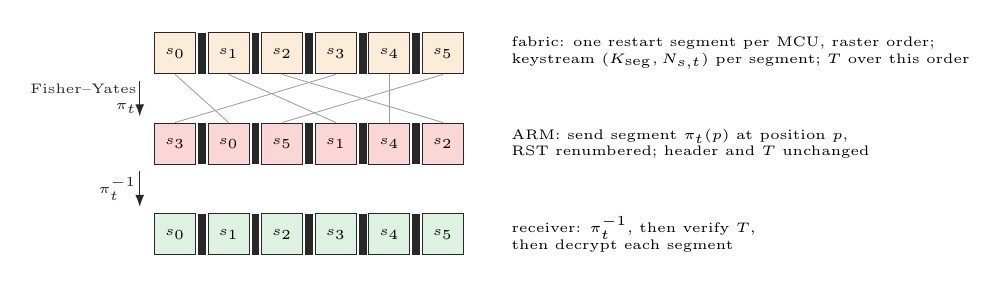
\begin{tikzpicture}[x=1cm, y=1cm,
  seg/.style={draw=inkc, minimum width=5.2mm, minimum height=5.2mm, inner sep=0pt, font=\tiny},
  rst/.style={fill=inkc, minimum width=1.0mm, minimum height=5.2mm, inner sep=0pt},
  st/.style={font=\tiny, align=left, anchor=west}]
\def\segrow#1#2#3{% #1 y, #2 list of labels, #3 fill
  \foreach \l [count=\i from 0] in {#2} {
    \node[seg, fill=#3] at (\i*0.68, #1) {$\l$};
    \ifnum\i<5 \node[rst] at (\i*0.68+0.34, #1) {};\fi
  }}
\segrow{0}{s_0,s_1,s_2,s_3,s_4,s_5}{plfill}
\node[st] at (4.15,0.0) {fabric: one restart segment per MCU, raster order;\\keystream $(K_{\mathrm{seg}}, N_{s,t})$ per segment; $T$ over this order};
\segrow{-1.15}{s_3,s_0,s_5,s_1,s_4,s_2}{cryfill}
\node[st] at (4.15,-1.15) {ARM: send segment $\pi_t(p)$ at position $p$,\\RST renumbered; header and $T$ unchanged};
\segrow{-2.3}{s_0,s_1,s_2,s_3,s_4,s_5}{rxfill}
\node[st] at (4.15,-2.3) {receiver: $\pi_t^{-1}$, then verify $T$,\\then decrypt each segment};
\draw[arr] (-0.45,-0.35) -- node[lbl, left, align=right]{Fisher--Yates\\$\pi_t$} (-0.45,-0.8);
\draw[arr] (-0.45,-1.5) -- node[lbl, left]{$\pi_t^{-1}$} (-0.45,-1.95);
\foreach \a/\b in {0/1,1/3,2/5,3/0,4/4,5/2} {
  \draw[inkc!45, line width=0.3pt] (\a*0.68,-0.27) -- (\b*0.68,-0.88);
}
\end{tikzpicture}
}
\caption{E5 in hardware form. The fabric codes one restart segment per MCU in raster order, each with its own keystream, and tags them in that order; the ARM sends segment $\pi_t(p)$ at wire position $p$; the receiver restores raster order before checking the tag. Black bars: restart markers.}
\label{fig:e5}
\end{figure}

\begin{enumerate}
\item the fabric codes every MCU $h = r \cdot (W/16) + c$ as its own restart segment, encrypted like E4 with keystream $Z_h$ of~\eqref{eq:zs}, and authenticates the segments in raster order with~\eqref{eq:tag} (level byte 5);
\item the ARM splits the scan at the restart markers and sends segment $\pi_t(p)$ at position $p$, renumbering the markers RST$_{p \bmod 8}$ in output order; headers, APP11 and tag are unchanged, and DRI = 1;
\item the receiver splits the received scan, restores raster order with $\pi_t^{-1}$, verifies $T_t$ and only then decrypts.
\end{enumerate}
The permutation is drawn from its own key, $K_\pi = \MAC_{K_e}(N(0,0,0), \text{``E5 MCU shuffle''})$, with the Fisher--Yates shuffle (Algorithm~\ref{alg:fy}) on the keystream of $(K_\pi, N(\sigma, t, 0))$; uniform indices come from rejection sampling.

\begin{algorithm}[t]
\caption{E5 order $\pi_t$ (ARM core and receiver)}
\label{alg:fy}
\begin{algorithmic}[1]
\Require $K_\pi$, $\sigma$, $t$, number of segments $M$
\State $Z \gets$ keystream of $(K_\pi, N(\sigma, t, 0))$; $\pi \gets (0, 1, \ldots, M-1)$
\For{$i = M-1$ \textbf{down to} $1$}
  \State $b \gets \lfloor \log_2 i \rfloor + 1$ \Comment{bits to express $i$}
  \Repeat \ $j \gets$ next $b$ bits of $Z$ \Until{$j \le i$}
  \State swap $\pi(i)$ and $\pi(j)$
\EndFor
\State \Return $\pi$ \Comment{wire position $p$ carries segment $\pi(p)$}
\end{algorithmic}
\end{algorithm}

\begin{proposition}[Uniform per-frame permutation]\label{prop:perm}
If the keystream bits are uniform and independent, Algorithm~\ref{alg:fy} returns each of the $M!$ permutations with probability $1/M!$, and it consumes on average
\begin{equation}
\bar n_\pi = \sum_{i=1}^{M-1} b_i \frac{2^{b_i}}{i+1} < 2 \sum_{i=1}^{M-1} b_i
\label{eq:fybits}
\end{equation}
keystream bits, $b_i = \lfloor \log_2 i \rfloor + 1$.
\end{proposition}
\begin{IEEEproof}
A $b_i$-bit draw is uniform on $\{0, \ldots, 2^{b_i} - 1\}$; conditioned on $j \le i$ it is uniform on $\{0, \ldots, i\}$, and the number of draws is geometric with success probability $(i+1)/2^{b_i} > 1/2$. Fisher--Yates with uniform $j \in \{0, \ldots, i\}$ at every step produces every permutation exactly once among the $\prod_{i=1}^{M-1}(i+1) = M!$ equally likely choice sequences.
\end{IEEEproof}
At 320$\times$240 ($M = \McuQVGA$) the permutation carries $\log_2 M! = \PermBitsQVGA$ bits of entropy and costs on average \FyBitsQVGA{} keystream bits (\FyRatioQVGA{} times the entropy); at 640$\times$480 ($M = \McuVGA$) $\log_2 M! = \PermBitsVGA$ bits and \FyBitsVGA{} keystream bits. The permutation changes with every frame because $t$ enters the nonce, so knowing the order of one frame tells nothing about the next; schemes with a fixed permutation fail exactly here (Section~\ref{sec:bench}).

\textit{Authentication of the order.} Because the tag covers the raster-order scan and the receiver computes $\pi_t^{-1}$ from the authenticated $(\sigma, t)$, moving, swapping, dropping or duplicating a segment on the wire changes the associated data of~\eqref{eq:tag} and the frame is rejected. Sending the frame unshuffled is also rejected, since the receiver always applies $\pi_t^{-1}$.

\textit{Equivalence.} An eavesdropper sees the same multiset of encrypted macroblocks at uniformly random positions as with a frame-level shuffle; the only difference is that each segment carries its own keystream instead of a slice of one frame keystream, which is invisible without the key. In our measurements the eavesdropper's pictures of both forms are pixel-identical (Section~\ref{sec:bench}).

\textit{Cost.} Each segment adds a two-byte marker, on average half a byte of padding, and loses DC prediction across macroblocks, so the overhead over E4 is roughly
\begin{equation}
\Delta B \approx M\bigl(2 + \tfrac12\bigr) + \Delta_{\mathrm{DC}} \ \text{bytes per frame},
\label{eq:e5cost}
\end{equation}
where $\Delta_{\mathrm{DC}}$ is the extra length of DC differences coded from zero. Measured, E5 costs \RiOverheadOneMin--\RiOverheadOneMax\,\% over E4 at 320$\times$240 (Section~\ref{sec:restart}); the fabric needs no frame buffer and no extra cipher core, and the ARM touches each output byte once.

\subsection{Authenticated feedback and the replay window}\label{sec:feedback}
The receiver returns a heartbeat every 0.5\,s and rate-limited alerts (tag failures, replays, malformed or stale frames, loss statistics). Feedback messages are Ascon-AEAD128 encrypted under $\Kfb$ with their own session and counter, so the attacker can neither read nor forge them, and they pass their own replay window. Both directions use the sliding window of SRTP~\cite{rfc3711} with 64 entries (Algorithm~\ref{alg:replay}). A frame older than the window, or seen before, is discarded; frames that arrive late but inside the window are accepted, which tolerates reordering on UDP. Frames older than the last frame shown are discarded as late without counting as replays, so that benign reordering does not raise alarms.

\begin{algorithm}[t]
\caption{Replay window (64 entries, after RFC~3711)}
\label{alg:replay}
\begin{algorithmic}[1]
\Require counter $t$; state: highest counter $\tau$, bitmap $w$
\If{$t > \tau$}
  \State $w \gets ((w \ll (t - \tau)) \lor 1) \bmod 2^{64}$; $\tau \gets t$; \Return accept
\EndIf
\State $o \gets \tau - t$
\If{$o \ge 64$ \textbf{or} bit $o$ of $w$ is set} \Return reject \EndIf
\State set bit $o$ of $w$; \Return accept
\end{algorithmic}
\end{algorithm}

\textit{Dead-man rule.} If no valid heartbeat arrives for 3\,s, the sender assumes that the feedback path is attacked: it switches to the highest level and rekeys (goal G4). Rekeys are rate-limited to one per 10\,s.

\subsection{Adaptive protection policies}\label{sec:policy}
The sender's ARM core collects evidence in one-second windows: tag failures $f_{\mathrm{int}}$, replays $f_{\mathrm{rep}}$, forged or replayed feedback $f_{\mathrm{fb}}$, junk floods $f_{\mathrm{fl}}$, the dead-man state $f_{\mathrm{dm}}$ and a loss level $f_{\mathrm{loss}} \in \{0, 1, 2\}$ (frame loss below 5\,\%, between 5 and 90\,\%, above 90\,\%) judged over three windows. It condenses them into a threat score
\begin{equation}
\theta = \min\bigl(1,\ f_{\mathrm{int}} + f_{\mathrm{rep}} + 0.8 f_{\mathrm{fb}} + 0.6 f_{\mathrm{fl}} + f_{\mathrm{dm}} + 0.25 f_{\mathrm{loss}}\bigr),
\label{eq:threat}
\end{equation}
shown on the dashboard and used by the bandit. Loss level 1 is reported as a degraded network, because more encryption cannot help against loss; only near-total suppression (level 2) counts as jamming. Two policies map evidence to a level, and neither goes below the configured minimum.

\textit{Threshold rule.} Any tag failure, replay, feedback attack or flood in a window raises the highest level and holds it for 8\,s after the evidence ends; suppression (loss level 2) does the same for 4\,s. Both policies share a safety layer: the dead-man rule, and a rekey when the tag failures of one window reach a configured burst size.

\textit{Contextual bandit.} The context $c$ is a small discrete vector of the evidence flags and whether an attack was seen in the last 30\,s; the action is a level $a$. After each window the bandit observes the loss
\begin{equation}
\ell(a) = \theta' \lambda(a) + w_c\, \kappa(a) + w_s [a \ne a_{\mathrm{prev}}],
\label{eq:loss}
\end{equation}
where $\theta'$ is the threat score of the next window, $\lambda(a)$ the measured edge correlation of level $a$, $\kappa(a)$ its fraction of encrypted bits, $w_c = 0.5$ and $w_s = 0.02$. It updates $Q(c, a) \leftarrow Q(c, a) + \eta \bigl(-\ell(a) - Q(c, a)\bigr)$ with $\eta = \max(0.05, 1/N(c,a))$ (sample average, then a floor), chooses an untried action first (optimistic initialization), and otherwise explores with probability $\varepsilon_c = 0.1/\sqrt{1 + n_c}$ and exploits $\arg\max_a Q(c, a)$~\cite{sutton2018}. Its table persists across episodes, so what it learned about an attack is used the next time the same context appears.

% =====================================================================================================
\section{Hardware Architecture}\label{sec:hardware}
\begin{figure*}[t]
\centering
\resizebox{\textwidth}{!}{% Fabric datapath of the contract-v3 lane encoder (rtl/secure_jpeg_lanes_top.v, rtl/encoder_lane.v).
% Bus widths are the RTL port widths; module names are the RTL file names.
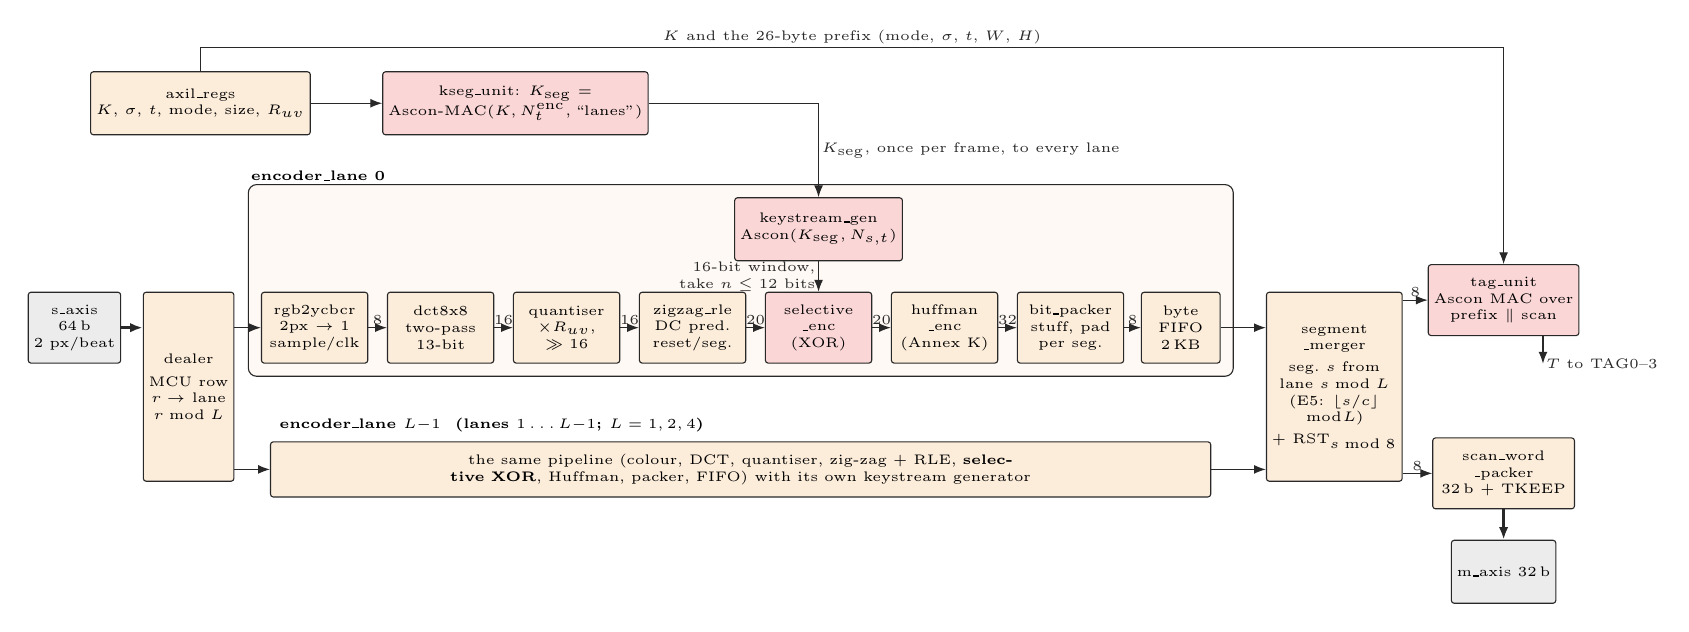
\begin{tikzpicture}[x=1cm, y=1cm, st/.style={pl, minimum height=9mm, minimum width=13.5mm, font=\tiny}]
% ---- input and dealer
\node[blk, fill=netfill, font=\tiny, minimum height=9mm] (in) at (0,0) {s\_axis\\64\,b\\2 px/beat};
\node[pl, font=\tiny, minimum height=24mm, minimum width=11mm, align=center] (deal) at (1.45,-0.75) {dealer\\[2pt]MCU row\\$r\to$ lane\\$r \bmod L$};
\draw[bus] (in) -- (in -| deal.west);
% ---- lane 0 (full) -- y = 0
\node[st] (cc0)  at (3.05,0) {rgb2ycbcr\\2px $\to$ 1\\sample/clk};
\node[st] (dct0) at (4.65,0) {dct8x8\\two-pass\\13-bit};
\node[st] (q0)   at (6.25,0) {quantiser\\$\times R_{uv}$,\\$\gg 16$};
\node[st] (zz0)  at (7.85,0) {zigzag\_rle\\DC pred.\\reset/seg.};
\node[st, fill=cryfill] (se0) at (9.45,0) {selective\\\_enc\\(XOR)};
\node[st] (hu0)  at (11.05,0) {huffman\\\_enc\\(Annex K)};
\node[st] (bp0)  at (12.65,0) {bit\_packer\\stuff, pad\\per seg.};
\node[st, minimum width=10mm] (ff0)  at (14.05,0) {byte\\FIFO\\2\,KB};
\node[cry, font=\tiny, minimum width=19mm, minimum height=8mm] (ks0) at (9.45,1.25) {keystream\_gen\\Ascon$(K_{\mathrm{seg}}, N_{s,t})$};
\draw[arr] (ks0) -- node[lbl, left, align=right]{16-bit window,\\take $n\le 12$ bits} (se0);
\draw[arr] (deal.east |- cc0) -- (cc0);
\draw[arr] (cc0) -- node[lbl, above]{8} (dct0);
\draw[arr] (dct0) -- node[lbl, above]{16} (q0);
\draw[arr] (q0) -- node[lbl, above]{16} (zz0);
\draw[arr] (zz0) -- node[lbl, above]{20} (se0);
\draw[arr] (se0) -- node[lbl, above]{20} (hu0);
\draw[arr] (hu0) -- node[lbl, above]{32} (bp0);
\draw[arr] (bp0) -- node[lbl, above]{8} (ff0);
\begin{scope}[on background layer]
\node[grp, fill=plfill!30, fit=(cc0)(ff0)(ks0), inner sep=1.6mm, label={[font=\tiny\bfseries, anchor=south west, inner sep=1pt]north west:encoder\_lane 0}] (lane0) {};
\end{scope}
% ---- lane L-1 (collapsed) -- y = -1.6
\node[pl, font=\tiny, text width=118mm, minimum height=7mm, align=center] (laneL) at (8.46,-1.8) {the same pipeline (colour, DCT, quantiser, zig-zag + RLE, \textbf{selective XOR}, Huffman, packer, FIFO) with its own keystream generator};
\node[font=\tiny\bfseries, anchor=south west] at (laneL.north west) {encoder\_lane $L{-}1$ \ (lanes $1 \ldots L{-}1$; $L = 1, 2, 4$)};
\draw[arr] (deal.east |- laneL) -- (laneL);
% ---- merger, tag, word packer
\node[pl, font=\tiny, minimum height=24mm, minimum width=13mm, align=center] (mrg) at (16.0,-0.75) {segment\\\_merger\\[2pt]seg.\ $s$ from\\lane $s \bmod L$\\(E5: $\lfloor s/c\rfloor$\\$\bmod L$)\\[2pt]+ RST$_{s \bmod 8}$};
\draw[arr] (ff0.east) -- (ff0.east -| mrg.west);
\draw[arr] (laneL.east) -- (laneL.east -| mrg.west);
\node[cry, font=\tiny, minimum width=18mm, minimum height=9mm] (tag) at (18.15,0.35) {tag\_unit\\Ascon MAC over\\prefix $\|$ scan};
\node[pl, font=\tiny, minimum width=18mm, minimum height=9mm] (wp) at (18.15,-1.85) {scan\_word\\\_packer\\32\,b + TKEEP};
\draw[arr] (mrg.east |- tag) -- node[lbl, above]{8} (tag.west);
\draw[arr] (mrg.east |- wp) -- node[lbl, above]{8} (wp.west);
\node[blk, fill=netfill, font=\tiny, minimum height=8mm] (out) at (18.15,-3.1) {m\_axis 32\,b};
\draw[bus] (wp) -- (out);
% ---- per-frame key, registers
\node[cry, font=\tiny, minimum width=24mm, minimum height=8mm] (kseg) at (5.6,2.85) {kseg\_unit: $K_{\mathrm{seg}}$ =\\Ascon-MAC$(K, N^{\mathrm{enc}}_t, \text{``lanes''})$};
\draw[arr] (kseg.east) -| node[lbl, pos=0.75, right]{$K_{\mathrm{seg}}$, once per frame, to every lane} (ks0.north);
\node[pl, font=\tiny, minimum width=24mm, minimum height=8mm] (regs) at (1.6,2.85) {axil\_regs\\$K$, $\sigma$, $t$, mode, size, $R_{uv}$};
\draw[arr] (regs) -- (kseg);
\draw[arr] (regs.north) -- ++(0,0.3) -| node[lbl, pos=0.25, above]{$K$ and the 26-byte prefix (mode, $\sigma$, $t$, $W$, $H$)} (tag.north);
\draw[arr] (tag.south) ++(0.5,0) -- ++(0,-0.35) node[lbl, right]{$T$ to TAG0--3};
\end{tikzpicture}
}
\caption{Fabric datapath of the lane encoder \texttt{secure\_jpeg\_lanes\_top} (module names are the RTL files; numbers on arrows are bus widths in bits). The dealer sends MCU row $r$ to lane $r \bmod L$; each lane converts two pixels per clock into one sample per clock, transforms, quantizes and entropy-codes its restart segments with its own keystream; the merger restores raster order and inserts restart markers; the tag unit authenticates the 26-byte prefix and the merged scan; the word packer writes 32-bit words to the DMA. The single-pipeline encoder \texttt{secure\_jpeg\_top} is one lane without dealer and merger, with one keystream per frame.}
\label{fig:pl}
\end{figure*}

\subsection{Datapath}\label{sec:datapath}
Fig.~\ref{fig:pl} shows the encoder. All stages are joined by valid/ready handshakes: data moves on a rising edge where both are high, a sender holds its data while valid is high and ready is low, and valid never depends on ready. Every stage therefore tolerates back-pressure from the DMA without losing or corrupting data, which the testbenches check with random stalls on every interface.

\textit{Colour conversion and line buffers.} \texttt{rgb2ycbcr\_2px} takes two pixels per clock from the 64-bit stream, applies~\eqref{eq:ycc} with three multiply-add trees per pixel (the luma line buffer is split into even and odd banks so that both pixels are written in one clock), averages chroma and writes an MCU row (16 lines) into block-RAM line buffers sized for 2048-pixel lines (1024 with four lanes). It reads the samples back block by block in the order Y0 Y1 Y2 Y3 Cb Cr, one sample per clock. Its buffers hold all block RAM of the encoder.

\textit{Transform and quantizer.} \texttt{dct8x8} computes~\eqref{eq:dct} as two passes of an eight-tap multiply-accumulate with a transpose buffer between them, one sample per clock; the row sums are pipelined over five stages. \texttt{quantiser} implements~\eqref{eq:quant} with one DSP multiplication by the reciprocal table, which the ARM writes through the register map once per session.

\textit{Zig-zag, run-length and DC coding.} \texttt{zigzag\_rle} stores the coefficients of a block in zig-zag order, takes the DC difference with one predictor per component, and emits symbols (is\_dc, run, $s$, $\amp$, EOB, component, frame-last), at most one per clock. Its predictors reset at every restart segment.

\textit{Encryption.} \texttt{selective\_enc} implements~\eqref{eq:selenc} (Section~\ref{sec:circuit}). \texttt{huffman\_enc} maps each symbol to a right-aligned chunk of up to 27 bits (code followed by the field) from the Annex~K tables, and \texttt{bit\_packer} assembles bytes, inserts the 0x00 after every 0xFF, and at the end of a segment pads with 1-bits and marks the last byte.

\textit{Merger, tag and output.} \texttt{segment\_merger} copies segment $s$ byte by byte from its lane's FIFO until the byte marked last, then writes 0xFF, 0xD0 $+ (s \bmod 8)$ unless $s$ is the last segment, and moves to the next lane. \texttt{tag\_unit} absorbs the prefix and every merged byte into an Ascon core; \texttt{scan\_word\_packer} packs bytes into 32-bit little-endian words with TKEEP and TLAST and counts them for the OUT\_BYTES register.

\subsection{Circuit of the encryption stage}\label{sec:circuit}
\begin{figure}[t]
\centering
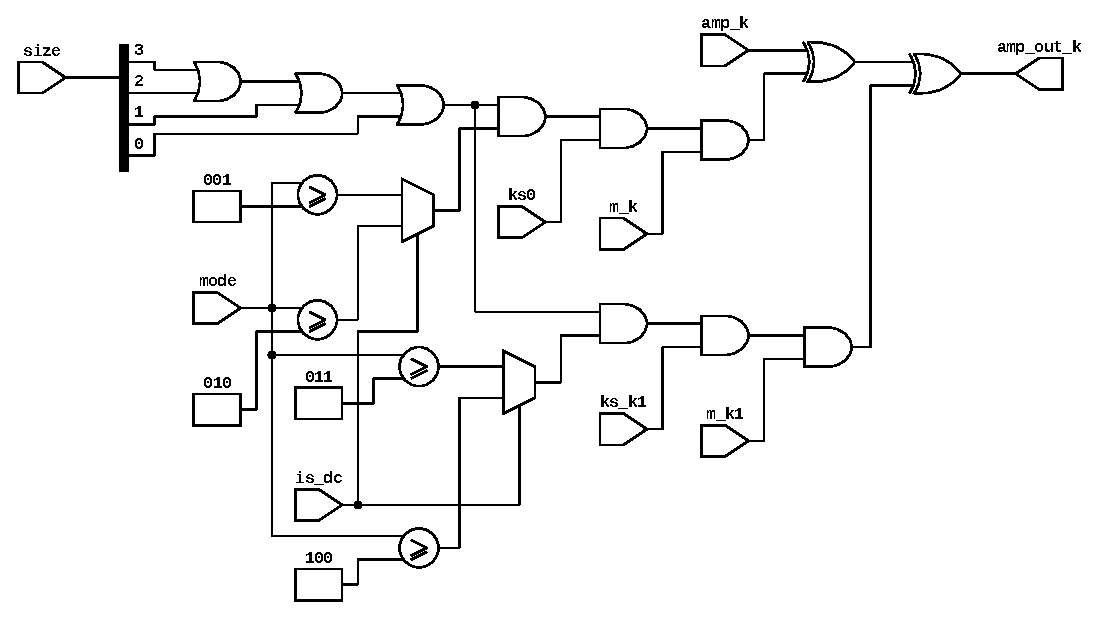
\includegraphics[width=\columnwidth]{figures/fig_selective_enc_bitslice.pdf}
\caption{Gate-level circuit of bit slice $k$ of \texttt{selective\_enc.v}, generated from the RTL by Yosys and netlistsvg. The OR of the size bits gives $[s \ne 0]$; comparators on the mode and two multiplexers selected by is\_dc form the sign enable $\gamma$ (upper path) and the amplitude enable $\alpha$ (lower path); the two XORs implement~\eqref{eq:slice}. $m_k = [k < s]$ and $m_{k+1}$ are bits of the mask $2^s - 1$; ks0 and ks\_k1 are bits 0 and $k{+}1$ of the keystream window. A test simulates the slice exhaustively and compares it with the golden model.}
\label{fig:circuit}
\end{figure}
Fig.~\ref{fig:circuit} is one bit slice of the stage at gate level, generated from its RTL; the handshake around it is described by the equations below. The control part decodes $\gamma = [s \ne 0] \wedge (\text{is\_dc} \mathbin{?} \text{mode} \ge 2 : \text{mode} \ge 1)$ and $\alpha = [s \ne 0] \wedge (\text{is\_dc} \mathbin{?} \text{mode} \ge 4 : \text{mode} \ge 3)$; mode 5 selects the same fields as mode 4 because all comparisons are $\ge$. The data part is eleven identical bit slices,
\begin{equation}
\amp'_k = \amp_k \xor (\gamma z_0 \wedge m_k) \xor (\alpha z_{k+1} \wedge m_{k+1}), \quad m = 2^s - 1,
\label{eq:slice}
\end{equation}
one XOR gate deep after the masks, so the stage closes timing with room to spare. The handshake accepts a symbol when $i_{\mathrm{ready}} = (\neg o_{\mathrm{valid}} \vee o_{\mathrm{ready}}) \wedge (k_{\mathrm{avail}} \ge n)$ and signals the keystream generator to advance by $n$ bits.

\textit{Keystream window.} \texttt{keystream\_gen} holds two 128-bit slots, the block being consumed ($u$) and the next one ($u'$), and a pointer $p \in [0, 127]$ to the next unused bit. It presents the 16-bit window $(u' \cat u) \gg p$ and its fill level $k_{\mathrm{avail}} = \min(16, 128 - p + 128\,[u' \text{ valid}])$; taking $n$ bits sets $p \leftarrow p + n$, and when $p$ passes 128 the next slot moves in. A new block is requested whenever fewer than two are held or in flight, so the core runs ahead of the consumer.

\begin{proposition}[The cipher never stalls the encoder]\label{prop:supply}
Once the first keystream block of a segment is available, the encryption stage never waits for keystream bits.
\end{proposition}
\begin{IEEEproof}
The stage accepts at most one symbol per clock and takes $n \le 11$ bits per symbol~\eqref{eq:need}, so the demand never exceeds 11 bits per cycle. The core produces 128 bits per data block in nine cycles (one cycle to absorb, eight rounds of $p^8$), i.e.\ $128/9 > 14$ bits per cycle, and it keeps up to 256 bits buffered, more than the 16 that the window exposes. Supply exceeds the worst-case demand, so the window, once filled, can never drop below the 11 bits a symbol needs.
\end{IEEEproof}
The first block costs an initialization ($p^{12}$, 12 cycles) and one data block (nine cycles). At the start of a frame this overlaps with filling the first MCU row (16 lines), so it is invisible; RTL simulation confirms that the cycle counts of E0--E4 differ by at most \MaxExtraCycles{} cycles per frame. In the lane encoder every segment restarts its keystream, and in E5 every MCU does; a segment of one MCU takes at least 384 cycles, so a 21-cycle restart overlapped with the previous segment costs a few per cent of throughput, which we measure in Section~\ref{sec:hwresults}.

\subsection{Ascon core}\label{sec:asconcore}
\begin{figure}[t]
\centering
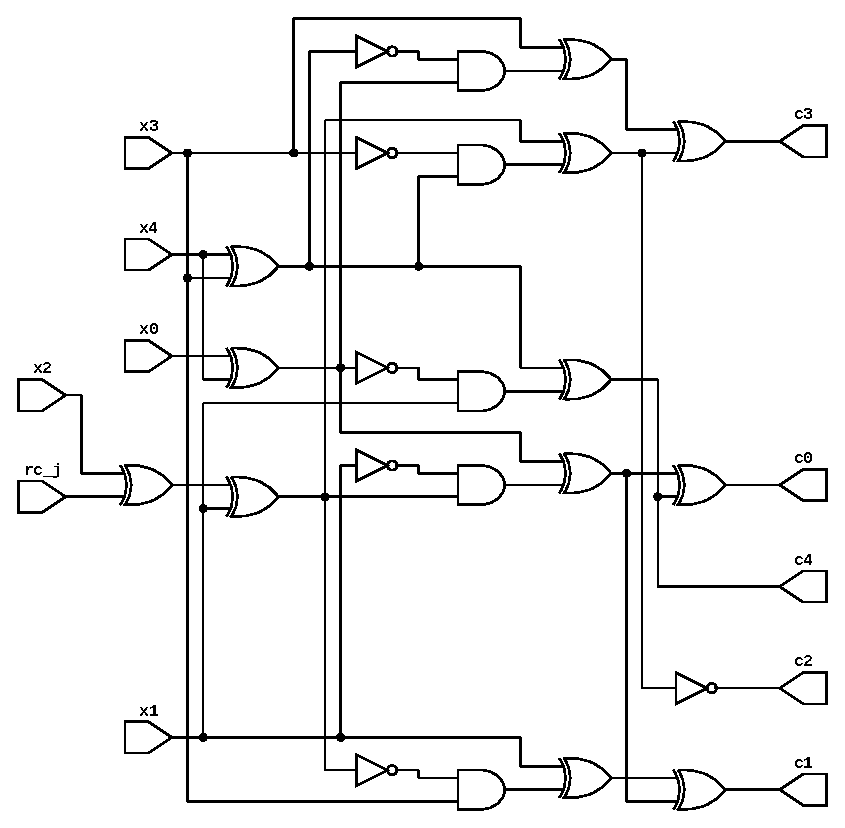
\includegraphics[width=\columnwidth]{figures/fig_ascon_sbox_slice.pdf}
\caption{One of the 64 bit slices of the Ascon round of \texttt{ascon\_round.v} ($p_C$ and $p_S$), generated from the RTL by Yosys and netlistsvg: twelve XOR (one for the round-constant bit rc\_j, zero for $j \ge 8$), five AND and six NOT gates. The linear layer $p_L$ acts on whole 64-bit words (two rotations and two XORs per bit). A test checks that 64 such slices followed by $p_L$ reproduce a round of the golden model.}
\label{fig:asconslice}
\end{figure}
\texttt{ascon\_aead128\_core} computes one round per clock cycle: a 320-bit state register, a 4-bit round counter $r$ and the combinational round of Fig.~\ref{fig:asconslice}, with the round constant $c = \bar r \cat r$ (eight bits, $\bar r$ the complement of $r$), which equals $16(15 - i) + i$ for round $i$. The $p^{12}$ permutation counts $r$ from 0 to 11, the $p^8$ permutation from 4 to 11. Counting the operators of \texttt{ascon\_round.v}, one bit slice of $p_S$ has 22 gates (eleven XOR, five AND, six NOT), so $p_S$ is $64 \times 22 = 1408$ gates, $p_L$ adds $2 \times 320$ two-input XORs and $p_C$ eight. A block interface accepts associated data and message blocks with byte masks and the padding rule of the standard; the same core serves as keystream generator (message blocks of zeros, never finalized), as MAC (associated data only, empty message) and as key-derivation unit. The design instantiates one core per lane for keystreams, one for the segment key and one for the tag.

\textit{Tag unit.} \texttt{tag\_unit} latches the 26-byte prefix at frame start, absorbs it, then gathers scan bytes into 128-bit blocks. A block of 16 bytes arrives in at least 16 cycles at one byte per clock, while absorbing it takes nine, so the tag unit never slows the merger; the final partial block, the empty message and the $p^{12}$ finalization add a fixed number of cycles after the last byte.

\subsection{Parallel lanes}\label{sec:lanes}
One pipeline consumes one sample per clock; with 1.5 samples per pixel it needs at least 1.5 cycles per pixel. Restart segments are independent (DC predictors reset, byte alignment, own keystream~\eqref{eq:zs}), so $L$ copies of the pipeline can code segments simultaneously: the dealer sends MCU row $r$ to lane $r \bmod L$ and the merger reads segment $s$ from lane $s \bmod L$ (in E5, segment $s$ belongs to MCU row $\lfloor s/c \rfloor$ with $c = W/16$ MCUs per row, so it comes from lane $\lfloor s/c \rfloor \bmod L$, tracked with row and column counters instead of a divider). The 64-bit input bus brings two pixels per clock. The cost per pixel is therefore bounded below by
\begin{equation}
c_L \ge \max\Bigl(\frac{1.5}{L}, \frac{1}{2}\Bigr), \qquad \Theta_L = \frac{f_{\mathrm{clk}}}{c_L},
\label{eq:lanes}
\end{equation}
i.e.\ \BoundOneCpp, \BoundTwoCpp{} and \BoundFourCpp{} cycles per pixel, or at most \BoundOneMpix, \BoundTwoMpix{} and \BoundFourMpix\,Mpixel/s at 100\,MHz for $L = 1, 2, 4$; beyond four lanes the input bus, not the encoder, is the limit. Two costs come on top. Before the first MCU row is complete no block can be transformed, which for a single pipeline gives the measured law
\begin{equation}
c_1(r) = 1.5 + \frac{A}{r}, \qquad A = \FillA,
\label{eq:fill}
\end{equation}
for a frame of $r$ MCU rows; and each segment adds a keystream restart and a byte flush. The bytes do not depend on $L$, because segments are merged in raster order and each one depends only on its own pixels and keystream.

\subsection{Register map and driver}\label{sec:regs}
\begin{table}[t]
\caption{AXI4-Lite register map (32-bit; \texttt{axil\_regs.v}).}
\label{tab:regs}
\centering\small\setlength{\tabcolsep}{3pt}
\begin{tabular}{lll}
\toprule
Offset & Name & Function \\
\midrule
0x00 & CTRL & bit 0 START (self-clearing), bits 3:1 level E0--E5 \\
0x04 & STATUS & DONE, BUSY, TAG\_VALID \\
0x08 & VERSION & 0x5EC0\_0200 (single pipeline); 0x5EC0\_03LL ($L$ lanes, bit 7 = E5) \\
0x10, 0x14 & WIDTH, HEIGHT & pixels (multiples of 16) \\
0x18, 0x50 & FRAME\_CTR (lo, hi) & 63-bit frame counter $t$ \\
0x1C, 0x4C & SESSION\_ID (lo, hi) & 64-bit session identifier $\sigma$ \\
0x20--0x2C & KEY0--3 & video key $K_e$ (write-only) \\
0x30 & OUT\_BYTES & scan bytes of the last frame \\
0x34--0x40 & TAG0--3 & tag $T_t$ \\
0x44, 0x48 & QT\_ADDR, QT\_DATA & 17-bit reciprocals $R(u, v)$ \\
\bottomrule
\end{tabular}
\end{table}
Table~\ref{tab:regs} gives the register map. Once per session the driver writes the key, the session identifier and the 128 reciprocals; per frame it writes the size and the counter, sets CTRL to $1 + 2 \cdot \text{level}$, starts the DMA receive and send channels, waits for DONE, and reads OUT\_BYTES and the tag. The VERSION register tells the driver which contract the bitstream implements: bit 7 says that the fabric codes E5 segments, and only then does the driver allow level E5.

\subsection{PYNQ-Z2 system}\label{sec:zynq}
\begin{figure*}[t]
\centering
\resizebox{\textwidth}{!}{% PYNQ-Z2 block design as built by future_work/board/block_design.tcl (cell names as in the Vivado
% utilisation report: ps7, ps7_axi_periph, axi_mem_intercon, dma, sjpeg, irq_concat, proc_sys_reset).
% Clock, reset and interrupt nets are drawn as net labels, as Vivado's diagram does.
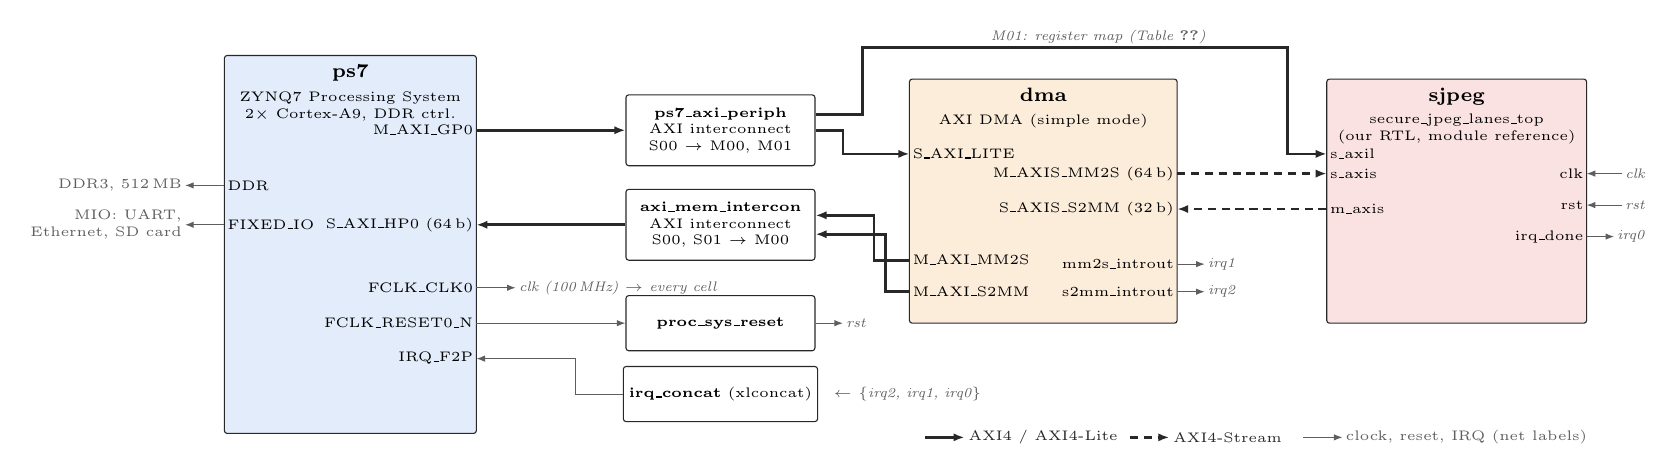
\begin{tikzpicture}[x=1cm, y=1cm,
  cell/.style={draw=inkc, fill=white, rounded corners=1pt, align=center, font=\tiny, inner sep=2pt},
  port/.style={font=\tiny, inner sep=1pt},
  net/.style={font=\tiny\itshape, inner sep=1pt, text=inkc!75},
  axi/.style={-{Latex[length=1.4mm]}, line width=1.0pt, inkc},
  axis/.style={-{Latex[length=1.4mm]}, line width=1.0pt, inkc, densely dashed},
  sg/.style={inkc!75, line width=0.4pt, -{Latex[length=1.1mm]}}]
% ---- PS7
\node[cell, fill=psfill, minimum width=32mm, minimum height=48mm] (ps) at (0,-0.15) {};
\node[font=\scriptsize\bfseries, anchor=north] at (ps.north) {ps7};
\node[font=\tiny, anchor=north, align=center] at ([yshift=-3.5mm]ps.north) {ZYNQ7 Processing System\\2$\times$ Cortex-A9, DDR ctrl.};
\coordinate (pGP) at (1.6,1.3);  \node[port, anchor=east] at (pGP) {M\_AXI\_GP0};
\coordinate (pHP) at (1.6,0.1);  \node[port, anchor=east] at (pHP) {S\_AXI\_HP0 (64\,b)};
\coordinate (pCK) at (1.6,-0.7); \node[port, anchor=east] at (pCK) {FCLK\_CLK0};
\coordinate (pRS) at (1.6,-1.15); \node[port, anchor=east] at (pRS) {FCLK\_RESET0\_N};
\coordinate (pIQ) at (1.6,-1.6); \node[port, anchor=east] at (pIQ) {IRQ\_F2P};
\coordinate (pDD) at (-1.6,0.6); \node[port, anchor=west] at (pDD) {DDR};
\coordinate (pFI) at (-1.6,0.1); \node[port, anchor=west] at (pFI) {FIXED\_IO};
\draw[sg] (pDD) -- ++(-0.5,0) node[port, left]{DDR3, 512\,MB};
\draw[sg] (pFI) -- ++(-0.5,0) node[port, left, align=right]{MIO: UART,\\Ethernet, SD card};
\draw[sg] (pCK) -- ++(0.5,0) node[net, right]{clk (100\,MHz) $\to$ every cell};
% ---- interconnects
\node[cell, minimum width=24mm, minimum height=9mm] (per) at (4.7,1.3) {\textbf{ps7\_axi\_periph}\\AXI interconnect\\S00 $\to$ M00, M01};
\node[cell, minimum width=24mm, minimum height=9mm] (mem) at (4.7,0.1) {\textbf{axi\_mem\_intercon}\\AXI interconnect\\S00, S01 $\to$ M00};
\draw[axi] (pGP) -- (per.west);
\draw[axi] (mem.west) -- (pHP);
% ---- DMA
\node[cell, fill=plfill, minimum width=34mm, minimum height=31mm] (dma) at (8.8,0.4) {};
\node[font=\scriptsize\bfseries, anchor=north] at (dma.north) {dma};
\node[font=\tiny, anchor=north] at ([yshift=-3.3mm]dma.north) {AXI DMA (simple mode)};
\coordinate (dL) at (7.1,1.0);   \node[port, anchor=west] at (dL) {S\_AXI\_LITE};
\coordinate (dM) at (7.1,-0.35);   \node[port, anchor=west] at (dM) {M\_AXI\_MM2S};
\coordinate (dS) at (7.1,-0.75);  \node[port, anchor=west] at (dS) {M\_AXI\_S2MM};
\coordinate (dA) at (10.5,0.75);  \node[port, anchor=east] at (dA) {M\_AXIS\_MM2S (64\,b)};
\coordinate (dB) at (10.5,0.3);  \node[port, anchor=east] at (dB) {S\_AXIS\_S2MM (32\,b)};
\coordinate (dI1) at (10.5,-0.4); \node[port, anchor=east] at (dI1) {mm2s\_introut};
\coordinate (dI2) at (10.5,-0.75); \node[port, anchor=east] at (dI2) {s2mm\_introut};
\draw[axi] (per.east) -- ++(0.35,0) |- (dL);
\draw[axi] (dM) -- ++(-0.45,0) |- ([yshift=1.2mm]mem.east);
\draw[axi] (dS) -- ++(-0.3,0) |- ([yshift=-1.2mm]mem.east);
\draw[sg] (dI1) -- ++(0.35,0) node[net, right]{irq1};
\draw[sg] (dI2) -- ++(0.35,0) node[net, right]{irq2};
% ---- our IP
\node[cell, fill=cryfill!70, minimum width=33mm, minimum height=31mm] (sj) at (14.05,0.4) {};
\node[font=\scriptsize\bfseries, anchor=north] at (sj.north) {sjpeg};
\node[font=\tiny, anchor=north, align=center] at ([yshift=-3.3mm]sj.north) {secure\_jpeg\_lanes\_top\\(our RTL, module reference)};
\coordinate (sL) at (12.4,1.0); \node[port, anchor=west] at (sL) {s\_axil};
\coordinate (sA) at (12.4,0.75);  \node[port, anchor=west] at (sA) {s\_axis};
\coordinate (sB) at (12.4,0.3);  \node[port, anchor=west] at (sB) {m\_axis};
\coordinate (sK) at (15.7,0.75);  \node[port, anchor=east] at (sK) {clk};
\coordinate (sR) at (15.7,0.35);  \node[port, anchor=east] at (sR) {rst};
\coordinate (sI) at (15.7,-0.05);  \node[port, anchor=east] at (sI) {irq\_done};
\draw[axis] (dA) -- (sA);
\draw[axis] (sB) -- (dB);
\draw[axi] ([yshift=2mm]per.east) -- ++(0.6,0) |- (11.9,2.35) |- (sL);
\node[net, anchor=south] at (9.5,2.35) {M01: register map (Table~\ref{tab:regs})};
\draw[sg] (sK) ++(0.45,0) node[net, right]{clk} -- (sK);
\draw[sg] (sR) ++(0.45,0) node[net, right]{rst} -- (sR);
\draw[sg] (sI) -- ++(0.35,0) node[net, right]{irq0};
% ---- reset and interrupt helpers
\node[cell, minimum width=24mm, minimum height=7mm] (rst) at (4.7,-1.15) {\textbf{proc\_sys\_reset}};
\draw[sg] (pRS) -- (rst.west);
\draw[sg] (rst.east) -- ++(0.35,0) node[net, right]{rst};
\node[cell, minimum width=24mm, minimum height=7mm] (cc) at (4.7,-2.05) {\textbf{irq\_concat} (xlconcat)};
\draw[sg] (cc.west) -- ++(-0.6,0) |- (pIQ);
\node[net, anchor=west] (cin) at ([xshift=1.5mm]cc.east) {$\leftarrow$ \{irq2, irq1, irq0\}};
% ---- legend
\draw[axi] (7.3,-2.6) -- ++(0.5,0) node[port, right]{AXI4 / AXI4-Lite};
\draw[axis] (9.9,-2.6) -- ++(0.5,0) node[port, right]{AXI4-Stream};
\draw[sg] (12.1,-2.6) -- ++(0.5,0) node[port, right]{clock, reset, IRQ (net labels)};
\end{tikzpicture}
}
\caption{Block design of the PYNQ-Z2 system as built by our script. The processing system clocks the fabric at 100\,MHz (FCLK\_CLK0), controls the DMA and the encoder over M\_AXI\_GP0 and an AXI interconnect, and gives the DMA access to DDR over the 64-bit high-performance port S\_AXI\_HP0. The DMA streams pixels into the encoder (64 bits, two pixels per beat) and scan words out of it (32 bits). Interrupts of the encoder and both DMA channels are concatenated into IRQ\_F2P; the reset block drives the encoder's active-high synchronous reset.}
\label{fig:zynq}
\end{figure*}
Fig.~\ref{fig:zynq} shows the system around the encoder. A script builds it in Vivado from the RTL (the encoder enters as a module reference, without packaging), runs synthesis, place and route and bitstream generation, and exports the hardware handoff file that the PYNQ framework reads to find the IP blocks by name. The DMA runs in simple (register) mode; the driver allocates physically contiguous buffers, copies a frame into the input buffer, and starts both channels. Everything in the system runs on one clock, which avoids clock-domain crossings.

\subsection{Timing closure}\label{sec:timing}
Three lessons from the Vivado runs are worth recording. The first implementation met timing in simulation but reached only about 47\,MHz after routing, because the DCT summed a full row in one clock; splitting the sums over five pipeline stages with a stall-able handshake restored 100\,MHz without changing an output bit. The second appeared only in the complete Zynq system: the DMA's output register fed the colour conversion, clamp and line-buffer write in one clock. Registering the pixel, the multiply-add sums and the clamped result moved the writes three clocks later in the same order. The third came with the lanes: the zig-zag stage, which formed the zig-zag address, read the block buffer, took the DC difference and derived the size category and field in one clock, had been the critical path of the single pipeline with tens of picoseconds of slack, and missed 100\,MHz in the two-lane system. Storing coefficients in zig-zag order and splitting the coding into two handshaked stages closed timing for every configuration and raised the encoder's slack to $+$\TopWns\,ns; at 125\,MHz the \TopLimitAtOneTwoFive{} is now the limit (WNS \TopWnsAtOneTwoFive\,ns). In all three cases the golden model was the referee: a fix was accepted only when every RTL test still matched it bit for bit.

% =====================================================================================================
\section{Verification Methodology}\label{sec:verification}
\textit{One referee.} A Python golden model implements Ascon, the integer transforms of Section~\ref{sec:background}, entropy coding, the encryption of~\eqref{eq:selenc}, the container, E5 and the receiver. Two views of it exist: a frame-level one used by the network simulation and the receiver, and a stage-level one whose functions match the RTL module boundaries; a test proves the two byte-identical on random frames for every level and both contracts (single pipeline and lanes). The Ascon model passes all 1089 known-answer tests of the official file for Ascon-AEAD128, and so does the RTL core. When the model and an RTL block disagree, the model is changed only if it contradicts T.81 or SP~800-232.

\textit{Block tests.} Every RTL module has a cocotb testbench that drives random inputs with random idle cycles and random back-pressure on every handshake and compares every output with the corresponding model function, reporting the first mismatch with its index, input, obtained and expected value. Throughput tests check one item per clock at full rate; mutation checks confirm that a stage which ignores back-pressure fails them.

\textit{System tests.} The complete encoders are compared byte for byte with the model for all levels, with 64-bit session identifiers and counters above $2^{32}$, for frames with fewer MCU rows than lanes, and under random stalls of both DMA streams; for the lane encoder with one, two and four lanes, including E5, where the test also runs the ARM permutation and the receiver. A self-checking Verilog-2001 testbench encodes stored frames in every level and is bit-exact with the model both in Icarus Verilog and in Vivado's simulator (XSim 2026.1). The board driver, the bit-exact board gate and the live sender are tested against an emulation of the bitstream that answers the register map with the model's bytes.

\textit{Bug log.} Every defect found, in the RTL, the model, the board scripts or the experiment scripts, received a regression test and an entry with its root cause and lesson. Table~\ref{tab:bugs} lists those that shaped the design. Two patterns recur: bit-exact simulation cannot reveal timing failures, and experiment scripts were wrong more often than the RTL.

\begin{table*}[t]
\caption{Defects that shaped the design (from our bug log).}
\label{tab:bugs}
\centering\small\setlength{\tabcolsep}{4pt}
\begin{tabular}{p{0.3\textwidth}p{0.33\textwidth}p{0.3\textwidth}}
\toprule
Symptom & Root cause & Consequence \\
\midrule
Two models gave different scans for one frame & sign rule, bit order, nonce layout and tag coverage had drifted & one contract, an equivalence test between the views \\
A level downgrade E2$\to$E1 went undetected & the tag covered the scan only & 26-byte authenticated prefix \eqref{eq:tag} \\
32-bit session identifiers & a repeat expected after about $2^{16}$ sessions & 64-bit $\sigma$, high-word registers \\
Field top-bit flip as ``sign'' & changed the magnitude too ($5 \to -6$) & exact negation, Lemma~\ref{lem:format} \\
47\,MHz after routing, all tests passing & a full DCT row summed in one clock & five-stage pipeline, post-route numbers in every claim \\
System missed timing, encoder alone met it & unconstrained input ports in the out-of-context run & I/O delays in every run \\
Board gate compared lanes with the wrong contract & reference chosen before the second contract existed & reference from the VERSION register \\
\bottomrule
\end{tabular}
\end{table*}

\textit{Results from data.} Every number in this paper is produced by a script from stored results and inserted by a generator, never typed; a test fails if a table in the manuscript differs from what the data produce, or if the text uses a number that the data do not define.

% =====================================================================================================
\section{Hardware Results}\label{sec:hwresults}
\subsection{Cycles and throughput}
% generated by paper/make_assets.py from paper/data -- do not edit
\begin{table}[t]
\caption{Encoder cycles per frame in RTL simulation (160x128, 100\,MHz). The last column extrapolates to 640$\times$480 at the same cycles per pixel.}
\label{tab:cycles}
\centering\small
\resizebox{\columnwidth}{!}{%
\begin{tabular}{lrrrr}
\toprule
Mode & Cycles & Cycles/pixel & $\Delta$ vs E0 & fps (640$\times$480) \\
\midrule
E0 & 33515 & 1.636 & +0 & 199 \\
E1 & 33517 & 1.637 & +2 & 199 \\
E2 & 33513 & 1.636 & -2 & 199 \\
E3 & 33517 & 1.637 & +2 & 199 \\
E4 & 33510 & 1.636 & -5 & 199 \\
\bottomrule
\end{tabular}}
\end{table}

In RTL simulation of a 160$\times$128 frame, the cycle counts of E0--E4 differ by at most \MaxExtraCycles{} cycles (Table~\ref{tab:cycles}), which is handshake noise rather than encryption work: as Proposition~\ref{prop:supply} predicts, encryption costs no cycles. Above the floor of 1.5 cycles per pixel, the only cost is filling the first MCU row: on \NumScaleSizes{} frame sizes the RTL follows~\eqref{eq:fill}, \CyclesPerPixel{} cycles per pixel at 160$\times$128 and \CppVGA{} at 640$\times$480 (Fig.~\ref{fig:throughput}).

\begin{figure}[t]
\centering
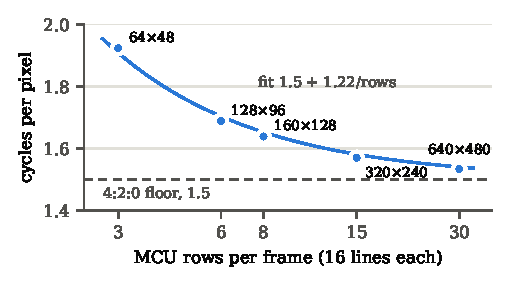
\includegraphics[width=\columnwidth]{figures/fig_throughput.pdf}
\caption{Cycles per pixel of the encoder RTL against frame height, measured in cycle-accurate simulation (dots), with the fitted law $1.5+\FillA/r$ of~\eqref{eq:fill} for $r$ MCU rows.}
\label{fig:throughput}
\end{figure}

\begin{figure}[t]
\centering
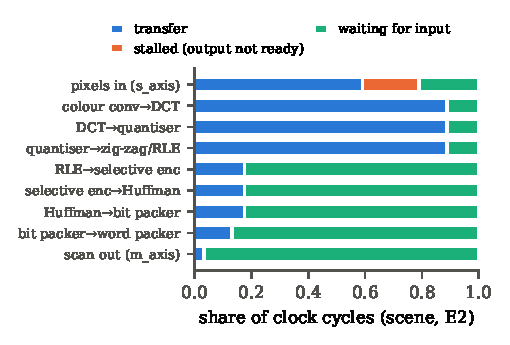
\includegraphics[width=\columnwidth]{figures/fig_stall.pdf}
\caption{Where the clock cycles go: share of cycles in which each handshake of the encoder pipeline transfers data, is stalled by its consumer, or waits for its producer (RTL simulation, synthetic scene, E2). Everything after the run-length coder, including the cipher, idles most of the time.}
\label{fig:stall}
\end{figure}
\textit{Where the cycles go.} Monitoring every handshake of the RTL pipeline over \ProfileCases{} cases (three images, three levels) shows the same cycles per pixel to within \ProfileCppSpread{} for every image and level, and an entropy path (run-length coding, encryption, Huffman coding, packing) that waits for data at least \EntropyIdle\,\% of the time (Fig.~\ref{fig:stall}). Faster designs must therefore widen the transform path, not the cipher, which is what the lanes do.

\textit{Lanes.} Measured at 100\,MHz on 640$\times$480 frames, bit-exact for every frame (Fig.~\ref{fig:lanesrtl}), one, two and four lanes reach \RtlOneLaneMpix, \RtlTwoLanesMpix{} and \RtlFourLanesMpix\,Mpixel/s (\RtlOneLaneCpp, \RtlTwoLanesCpp{} and \RtlFourLanesCpp{} cycles per pixel), against the bounds \BoundOneMpix, \BoundTwoMpix{} and \BoundFourMpix{} of~\eqref{eq:lanes}. Four lanes give \RtlFourLanesSpeedup$\times$ the single pipeline, \RtlFourLanesFps{} frames/s at 640$\times$480 or \RtlFourLanesHdFps{} at 1080p, above the \mbox{150\,Mpixel/s} that the commercial encoder of~\cite{logijpge} reports at 150\,MHz without any cryptography, at two thirds of its clock. The gap to the bound has two causes: a frame starts only after the previous one is done, so every frame pays~\eqref{eq:fill} once, and each segment adds a keystream restart and a byte flush. An event model that also lets the next frame's first MCU row arrive early projects \ProjTwoLanesMpix{} and \ProjFourLanesMpix\,Mpixel/s (Fig.~\ref{fig:lanes}). The latency from the first pixel to the first scan word is \RtlFourLanesLatUs\,$\mu$s (\RtlFourLanesLatLines{} lines of a 640$\times$480 frame) for any number of lanes: the 16 lines of the first MCU row plus the pipeline. E5, with one restart per MCU, costs a few per cent of throughput in the lane encoder. Two build options trade along other axes. With camera-native YUYV input (four pixels per beat, Section~\ref{sec:lanes}) four lanes reach \YuyvFourLanesMpix\,Mpixel/s (\YuyvFourLanesCpp{} cycles per pixel) and read \YuyvFourLanesInMBs\,MB/s from DDR instead of \RtlFourLanesInMBs; with one line-buffer set per lane instead of two, four lanes keep \NbufOneFourLanesMpix\,Mpixel/s (\NbufOneFourLanesCpp{} cycles per pixel) on half the converter memory, which is what lets four lanes take 1080p lines on this device.

\begin{figure}[t]
\centering
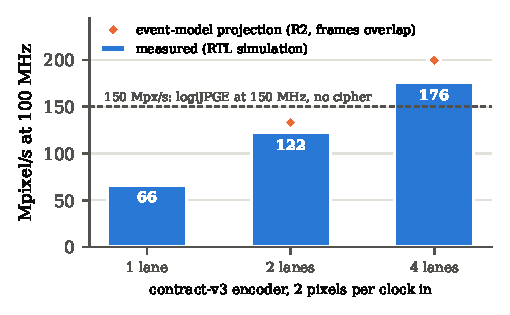
\includegraphics[width=\columnwidth]{figures/fig_lanes_rtl.pdf}
\caption{Throughput of the lane encoder, 640$\times$480 frames at 100\,MHz, measured in cycle-accurate simulation with every frame bit-exact against the golden model (bars), next to the event-model projection with overlapping frames (diamonds) and the published figure of a commercial encoder without cryptography~\cite{logijpge} (dashed).}
\label{fig:lanesrtl}
\end{figure}
\begin{figure}[t]
\centering
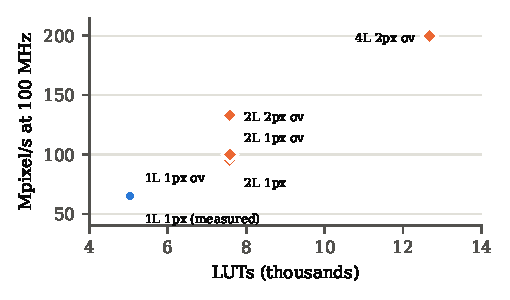
\includegraphics[width=\columnwidth]{figures/fig_lanes.pdf}
\caption{Projected throughput at 100\,MHz against LUTs for 640$\times$480 frames (event model calibrated on the measured RTL law). Labels: $L$ lanes, pixels per clock at the input, ``ov'': the next frame overlaps the current one; the circle is the measured single pipeline.}
\label{fig:lanes}
\end{figure}

\subsection{Area, timing and power}
% generated by paper/make_assets.py from paper/data -- do not edit
\begin{table}[t]
\caption{Resources on the xc7z020 (53\,200 LUT, 106\,400 FF, 140 BRAM36, 220 DSP). Source: Vivado post-route, out of context, 100\,MHz with I/O delays of 20\,\% of the period, WNS +0.630\,ns.}
\label{tab:resources}
\centering\small
\resizebox{\columnwidth}{!}{%
\begin{tabular}{lrrrr}
\toprule
Block & LUT & FF & BRAM36 & DSP \\
\midrule
Encoder (all) & 4785 (9.0\%) & 3051 (2.9\%) & 25.5 (18.2\%) & 23 (10.4\%) \\
\quad colour conversion + line buffers & 459 & 220 & 25 & 0 \\
\quad DCT and quantizer & 806 & 69 & 0 & 22 \\
\quad zig-zag, Huffman, packing & 717 & 323 & 0 & 0 \\
\quad keystream generator (Ascon) & 949 & 851 & 0 & 0 \\
\quad tag unit (Ascon) & 1358 & 1072 & 0 & 0 \\
\quad selective encryption & 82 & 24 & 0 & 0 \\
\quad AXI-Lite registers & 392 & 451 & 0 & 0 \\
\bottomrule
\end{tabular}}
\end{table}

After place and route in Vivado the single-pipeline encoder meets \TopMhz\,MHz on the xc7z020 (WNS $+$\TopWns\,ns, out of context, I/O delays of 20\,\% of the period), i.e.\ \TopMpix\,Mpixel/s or \FpsVGA{} frames/s at 640$\times$480. Table~\ref{tab:resources} gives the resources (\TopLuts{} LUTs, \TopLutPct\,\% of the device). The two Ascon instances take \CryptoLutShare\,\% of the LUTs; the selective-encryption stage itself is tiny; all \ConvBram{} BRAM36 are the converter's line buffers for 2048-pixel lines. With switching activity from simulating a real frame (SAIF), the encoder draws about \SaifTopMw\,mW; the vectorless estimate is \TopPowerMw\,mW. Two lanes take \TwoLanesLuts{} LUTs, \TwoLanesBram{} BRAM36 and \TwoLanesDsp{} DSPs (WNS $\TwoLanesWns$\,ns), four lanes \FourLanesLuts{} LUTs, \FourLanesBram{} BRAM36 and \FourLanesDsp{} DSPs (WNS $\FourLanesWns$\,ns, lines up to 1024 pixels). E5 adds no BRAM or DSP; with two lanes it draws \SaifLanesEfiveMw\,mW against \SaifLanesEtwoMw\,mW for E2. Out of context the single pipeline and two lanes also meet 125\,MHz (WNS \TopWnsAtOneTwoFive{} and \LanesTwoWnsAtOneTwoFive\,ns, Section~\ref{sec:hardware}). All three complete PYNQ-Z2 systems close timing at 100\,MHz: the single pipeline with \OverlayLuts{} LUTs (WNS $\OverlayWns$\,ns), two lanes on a 64-bit pixel stream with \OverlayLanesLuts{} LUTs (WNS $\OverlayLanesWns$\,ns), and four lanes with \OverlayLanesFourLuts{} LUTs, \OverlayLanesFourBram{} BRAM36 and \OverlayLanesFourDsp{} DSPs (WNS $\OverlayLanesFourWns$\,ns, \OverlayLanesFourLutPct\,\% of the LUTs); Vivado estimates \OverlayPowerW, \OverlayLanesPowerW{} and \OverlayLanesFourPowerW\,W for the complete systems, dominated by the processing system.

% generated by paper/make_assets.py from paper/data -- do not edit
\begin{table}[t]
\caption{Comparison with published FPGA designs. Their numbers are as reported by each source; ours are
post-route (Table~\ref{tab:resources}) with throughput from the RTL cycle count. Mpx/s: million pixels per second.}
\label{tab:compare}
\centering\small
\resizebox{\columnwidth}{!}{%
\begin{tabular}{llrrrrrl}
\toprule
Design & Device & LUT & BRAM & DSP & MHz & Mpx/s & Crypto \\
\midrule
Ours: encoder & Zynq-7020 & 5{,}039 & 24.5 & 23 & 100 & 61 & sel.\ AEAD \\
Ours: one Ascon & Zynq-7020 & 860--969 & 0 & 0 & 100 & -- & AEAD core \\
logiJPGE~\cite{logijpge} & Zynq-7020 & 3{,}240 & 16 & 30 & 150 & 150 & none \\
CAST JPEG-E-S~\cite{castjpeg} & Artix-7 & 3{,}069 & 2 & 16 & 166 & -- & none \\
Khairallah~\cite{khairallah2023} & Artix-7 & 1{,}031 & 0 & 0 & 200 & -- & MAC \\
Kurian~\cite{kurian2025} & Artix-7 & 5{,}335 & 32 & 0 & 100 & -- & AEAD \\
\bottomrule
\end{tabular}}
\end{table}

% generated by paper/make_assets.py from paper/data -- do not edit
\begin{table}[t]
\caption{Hardware figures of merit at 100\,MHz, 640$\times$480, E2: throughput from cycle-accurate RTL simulation (no DMA stalls), area and power post-route. Energy per pixel = on-chip power / throughput.}
\label{tab:hweff}
\centering\small\setlength{\tabcolsep}{2.5pt}
\resizebox{\columnwidth}{!}{%
\resizebox{\columnwidth}{!}{%
\begin{tabular}{lrrrrrrr}
\toprule
Design & LUT & Mpx/s & Mpx/s per kLUT & Gbit/s in & fps 1080p & Power (mW) & nJ/pixel \\
\midrule
Ours{,} single pipeline (v2) & 5{,}037 & 65 & 12.9 & 1.56 & 31 & 210 (SAIF) & 3.22 \\
Ours{,} 2 lanes & 10{,}069 & 122 & 12.1 & 2.94 & 59 & 319 (SAIF) & 2.61 \\
Ours{,} 4 lanes & 16{,}893 & 176 & 10.4 & 4.22 & 85 & 555 (vectorless) & 3.16 \\
\bottomrule
\end{tabular}}}
\end{table}


\subsection{Comparison}
Table~\ref{tab:compare} sets the design against published FPGA work. Each of our Ascon cores (\AsconLutMin--\AsconLutMax{} LUTs) is as small as the round-per-cycle Ascon-p cores of~\cite{khairallah2023}; our JPEG datapath without the cipher (colour conversion, transform, quantizer and entropy coder in Table~\ref{tab:resources}) uses fewer LUTs than the commercial encoders~\cite{logijpge,castjpeg}, which however process one sample per clock at 150--166\,MHz with less block RAM and no cryptography. Table~\ref{tab:hweff} gives the figures of merit that hardware papers compare: \HeTopPerKlut, \HeTwoPerKlut{} and \HeFourPerKlut\,Mpixel/s per thousand LUTs for one, two and four lanes, against \HeKishorePerKlut{} for the scrambling encoder of Kishore et al.~\cite{kishore2015} and \HeLogiPerKlut{} for the commercial encoder without cryptography~\cite{logijpge}; and \HeTopNj, \HeTwoNj{} and \HeFourNj\,nJ per pixel. One Ascon core accepts a 128-bit block every \AsconCyclesPerBlock{} clocks once initialized (eight rounds and one handshake, measured in RTL), i.e.\ \AsconGbps\,Gbit/s at 100\,MHz or \AsconGbpsPerKlut\,Gbit/s per thousand LUTs of the larger instance; the selective encryption needs far less, since it consumes at most one sign bit and the amplitude bits of each non-zero coefficient. The lanes buy throughput, not efficiency: each lane carries its own transform and line buffers, so area grows with $L$ while the energy per pixel stays roughly constant.

\subsection{Board evaluation}\label{sec:board}
% generated by paper/make_assets.py from paper/data -- do not edit
\begin{table*}[t]
\caption{On the PYNQ-Z2 (24 Oct 2026): the final board images, each at the clock it was built for, and the same
function on the board's ARM Cortex-A9. Bit-exact: every frame of every level compared byte for byte (scan and tag)
with the golden model running on the board (58 frames in all). Fabric: START to DONE from
the encoder's CYCLES register for one 640$\times$480 frame (Mpixel/s in brackets); wait: share of those cycles in
which the encoder could take a pixel but the DMA had none, mostly because the Python driver starts the DMA after the encoder. Frame: a complete authenticated JPEG with headers (and
for E5 the segment order) on the ARM, the pixels already in the DMA buffer as a camera would leave them, median of
50 frames (frames/s in brackets). ARM rows: median of 30 frames; ``file'' encrypts the whole JPEG, so it does not
play without the key.}
\label{tab:board}
\centering\small\setlength{\tabcolsep}{4pt}
\resizebox{\textwidth}{!}{%
\begin{tabular}{lrlrrrr}
\toprule
Encoder & MHz & Bit-exact & Fabric, ms & Wait (\%) & E2 frame, ms & E5 frame, ms \\
\midrule
4 lanes & 125 & E0--E5 & 1.97 (156) & 31 & 5.9 (169) & 8.4 (119) \\
2 lanes & 100 & E0--E5 & 3.06 (100) & 21 & 7.0 (144) & 9.8 (102) \\
1 lane & 100 & E0--E4 & 5.34 (58) & 12 & 9.2 (108) & -- \\
\midrule
ARM, ours in C, 1 core & -- & E0--E5 & -- & -- & 114.2 (8.8) & 133.0 (7.5) \\
ARM, ours in C, 2 cores & -- & E0--E5 & -- & -- & 61.6 (16.2) & 74.8 (13.4) \\
ARM, libjpeg-turbo, no security & -- & -- & -- & -- & 28.8 (34.8) & -- \\
ARM, libjpeg-turbo + Ascon (file) & -- & -- & -- & -- & 31.7 (31.5) & -- \\
ARM, libjpeg-turbo + AES-GCM (file) & -- & -- & -- & -- & 31.9 (31.3) & -- \\
\bottomrule
\end{tabular}}
\end{table*}

Following the practice of Section~\ref{sec:evalpractice}, the board evaluation on the PYNQ-Z2 has four parts, all scripted and rehearsed against an emulation of the bitstream: (A1) a bit-exact gate that encodes frames of two sizes in every level on the fabric and compares every byte and tag with the golden model; (A2) the encode time with registers and DMA, and the full frame time including the ARM's headers; (A3) the same function on the board's processing system: our encoder compiled in C for the Cortex-A9, gated bit-exact against the golden model in every level and run on one and both cores (contract-v3 segments are independent, so the two cores act like two lanes), next to libjpeg-turbo alone and with whole-file Ascon-AEAD128 or AES-GCM, the fair baseline because that core has no AES instructions; and (A4) power from an inline meter, idle and under each workload, giving energy per frame. Parts A1 and A2 are done (Table~\ref{tab:board}). The two-lane E5 bitstream, rebuilt after one defect in the block design (the DMA's write master was left unconnected; Table~\ref{tab:bugs} lists the lesson), is bit-exact with the golden model in every level \BoardModes{} at \BoardSizes{}: \BoardFramesTotal{} frames, every scan byte and every tag. The board thus confirms Lemma~\ref{lem:format} and the lane, E5 and tag logic on silicon, not only in simulation. With our Python driver a 640$\times$480 frame takes \BoardMsVGA\,ms (\BoardFpsVGA{} frames/s; \BoardFpsQVGA{} at 320$\times$240), and the times of E0--E4 differ by at most \BoardSpreadMsVGA\,ms: on silicon too, encryption costs no time. That time is dominated by the ARM, which converts and copies every pixel into the DMA buffer and flushes the cache, not by the fabric, which needs \RtlTwoLanesVgaMs\,ms per frame in RTL simulation; E5 adds \BoardEfiveExtraMsVGA\,ms for splitting and reordering the segments on the ARM. The rebuilt bitstream adds three counters to the register map (clocks from start to done, clocks waiting for pixels, clocks stalled by the output DMA), so the fabric-only time is read from the silicon itself, and the driver now writes the pixels straight into the DMA buffer and maintains the cache only over the frame's bytes. \TODO{A2 fabric-only time from the counters and the new driver, A3 PS baseline (future\_work/arm/arm\_baseline.py), A4 measured power and energy per frame.}

% =====================================================================================================
\section{Security Evaluation}\label{sec:security}
\subsection{Setup}
We measure what a keyless observer can reconstruct. For every frame we take the better of two pictures: the protected stream decoded as is, and a \emph{replacement attack} that substitutes fixed guesses for the encrypted values (absolute values for encrypted signs, the smallest value of the size category for encrypted amplitudes, zero DC differences) and re-encodes a valid JPEG. Leakage is the edge correlation~\eqref{eq:edge} of this picture with the original; we also report SSIM~\cite{ssim}. Sources are a synthetic corridor scene; \NumClips{} clips that we analyse but do not reproduce (two film trailers, two talking-head videos and a handheld phone video, identified by hash); \NumOpenClips{} openly licensed films of the Blender Foundation, the Sintel trailer and Tears of Steel (CC~BY~3.0)\footnote{\url{https://durian.blender.org}, \url{https://mango.blender.org}}; and the 24 images of the Kodak set\footnote{\url{http://r0k.us/graphics/kodak/}}. Video is resized to 320$\times$240 and sampled every 150 frames; frames without edges are excluded.

\textit{Format compliance.} The protected streams of \AllDecode{} six levels decode without error in \Decoders{}, at the original resolution, as Lemma~\ref{lem:format} requires.

\subsection{Outline leakage}\label{sec:leakage}
\begin{figure*}[t]
\centering
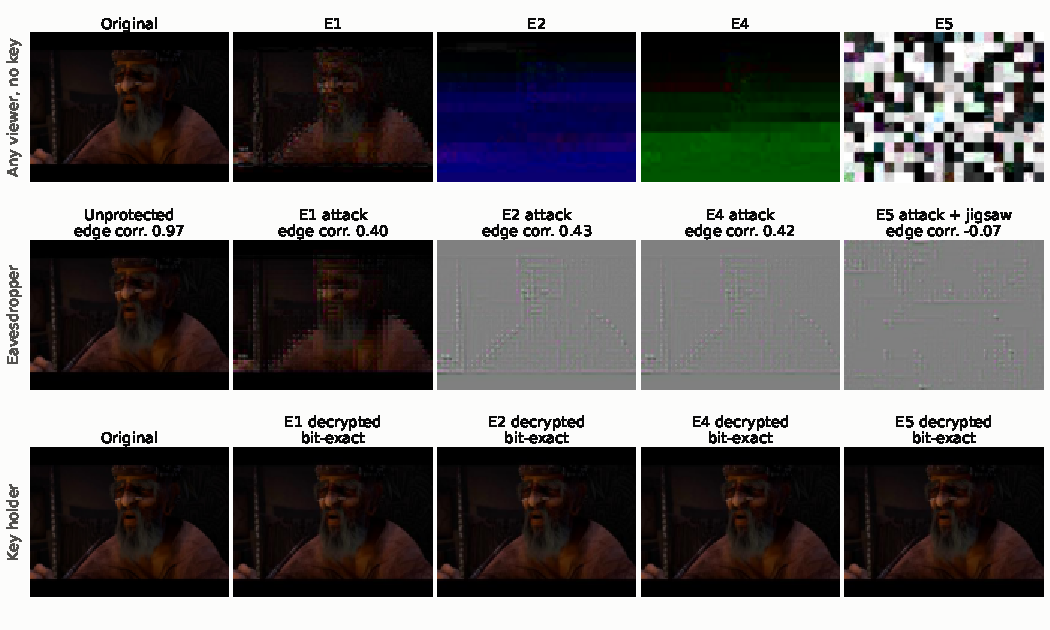
\includegraphics[width=0.66\textwidth]{figures/fig_visual_grid.pdf}
\caption{One frame of the Sintel trailer (\copyright{} Blender Foundation, CC~BY~3.0) per protection level. Top: what any viewer shows without the key. Middle: the eavesdropper's best reconstruction (replacement attack; for E5 followed by the jigsaw solver) with its edge correlation. Bottom: the key holder's output, bit-exact with the unprotected encoder.}
\label{fig:grid}
\end{figure*}
% generated by paper/make_assets.py from paper/data -- do not edit
\begin{table}[t]
\caption{Outline leakage: edge correlation between the original and the eavesdropper's best keyless reconstruction (decode or replacement attack; 0 = no outline), up to 20 frames per source; frames without edges are skipped. The first row is the fraction of payload bits encrypted.}
\label{tab:leakage}
\centering\small\setlength{\tabcolsep}{4pt}
\resizebox{\columnwidth}{!}{%
\begin{tabular}{lrrrrrr}
\toprule
Source & E0 & E1 & E2 & E3 & E4 & E5 \\
\midrule
Enc.\ share & 0.00 & 0.11 & 0.13 & 0.26 & 0.30 & 0.31 \\
\midrule
Synthetic & 1.00 & 0.38 & 0.36 & 0.37 & 0.37 & 0.00 \\
Trailer A & 0.99 & 0.47 & 0.34 & 0.34 & 0.33 & 0.01 \\
Trailer B & 0.99 & 0.58 & 0.27 & 0.31 & 0.30 & 0.02 \\
Talk A & 0.99 & 0.50 & 0.44 & 0.44 & 0.44 & -0.00 \\
Talk B & 0.99 & 0.49 & 0.38 & 0.44 & 0.43 & 0.01 \\
Sintel & 0.99 & 0.35 & 0.25 & 0.26 & 0.27 & -0.00 \\
Tears of Steel & 0.99 & 0.47 & 0.34 & 0.35 & 0.43 & -0.01 \\
Kodak & 0.99 & 0.39 & 0.32 & 0.33 & 0.30 & 0.00 \\
\bottomrule
\end{tabular}}
\end{table}

Fig.~\ref{fig:grid} and Table~\ref{tab:leakage} show the main effect. Under E1--E4 the eavesdropper sees a clear outline of the scene: edge correlation stays between \LeakEOneFourMin{} and \LeakEOneFourMax{} on the real sources, and encrypting amplitudes in addition to signs (E3, E4) does not reduce it, because the positions and size categories of the non-zero coefficients remain public (Lemma~\ref{lem:format}). The keyed macroblock permutation of E5 removes the outline (edge correlation between \LeakEFiveMin{} and \LeakEFiveMax). In terms of cost, E2 encrypts \CostEtwo\,\% of the payload bits, E4 \CostEfour\,\%, and E5 only slightly more, \CostEfive\,\%, yet only E5 moves leakage to zero.

% generated by paper/make_assets.py from paper/data -- do not edit
\begin{table}[t]
\caption{Edge correlation of the eavesdropper's best keyless picture with 95\,\% bootstrap intervals over the frames of each source (last column: frames).}
\label{tab:leakage_ci}
\centering\small\setlength{\tabcolsep}{3pt}
\resizebox{\columnwidth}{!}{%
\begin{tabular}{lccccr}
\toprule
Source & E1 & E2 & E4 & E5 & $n$ \\
\midrule
Synthetic & 0.38 {\scriptsize[0.37, 0.38]} & 0.36 {\scriptsize[0.36, 0.37]} & 0.38 {\scriptsize[0.37, 0.38]} & 0.00 {\scriptsize[-0.01, 0.00]} & 60 \\
Trailer A & 0.47 {\scriptsize[0.46, 0.49]} & 0.30 {\scriptsize[0.26, 0.34]} & 0.28 {\scriptsize[0.24, 0.33]} & 0.01 {\scriptsize[0.01, 0.02]} & 60 \\
Trailer B & 0.56 {\scriptsize[0.54, 0.58]} & 0.34 {\scriptsize[0.30, 0.38]} & 0.32 {\scriptsize[0.28, 0.36]} & 0.01 {\scriptsize[0.01, 0.02]} & 60 \\
Talk A & 0.51 {\scriptsize[0.49, 0.52]} & 0.45 {\scriptsize[0.42, 0.47]} & 0.44 {\scriptsize[0.42, 0.46]} & 0.01 {\scriptsize[0.00, 0.01]} & 60 \\
Talk B & 0.49 {\scriptsize[0.47, 0.51]} & 0.40 {\scriptsize[0.36, 0.43]} & 0.40 {\scriptsize[0.38, 0.43]} & 0.01 {\scriptsize[0.00, 0.01]} & 60 \\
Phone A & 0.45 {\scriptsize[0.44, 0.46]} & 0.35 {\scriptsize[0.32, 0.37]} & 0.33 {\scriptsize[0.31, 0.36]} & 0.00 {\scriptsize[0.00, 0.01]} & 60 \\
Sintel & 0.35 {\scriptsize[0.30, 0.41]} & 0.29 {\scriptsize[0.25, 0.33]} & 0.28 {\scriptsize[0.25, 0.31]} & -0.01 {\scriptsize[-0.01, 0.00]} & 25 \\
Tears of Steel & 0.45 {\scriptsize[0.42, 0.47]} & 0.35 {\scriptsize[0.30, 0.39]} & 0.35 {\scriptsize[0.30, 0.39]} & -0.01 {\scriptsize[-0.01, 0.00]} & 60 \\
Kodak & 0.39 {\scriptsize[0.36, 0.42]} & 0.33 {\scriptsize[0.27, 0.38]} & 0.31 {\scriptsize[0.27, 0.35]} & 0.00 {\scriptsize[0.00, 0.01]} & 24 \\
\bottomrule
\end{tabular}}
\end{table}

\begin{figure}[t]
\centering
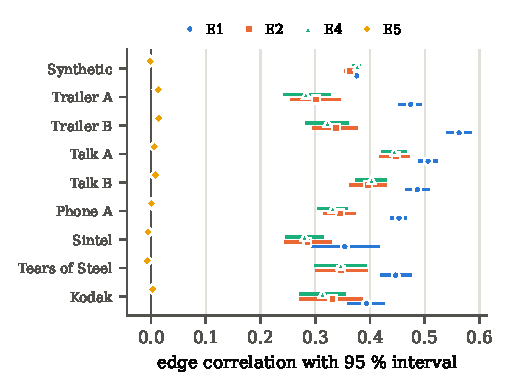
\includegraphics[width=\columnwidth]{figures/fig_leakage_ci.pdf}
\caption{Edge correlation of the eavesdropper's best keyless picture per source and level, with 95\,\% bootstrap intervals over up to \LeakFramesMax{} frames. E5's intervals lie at zero on every source; E1--E4 leak an outline everywhere.}
\label{fig:leakage_ci}
\end{figure}
\textit{Statistical confidence.} Table~\ref{tab:leakage_ci} and Fig.~\ref{fig:leakage_ci} give every leakage value with a 95\,\% percentile-bootstrap interval over the frames of its source. The intervals of E1--E4 are narrow and far from zero on all sources, so the outline leakage is not an effect of a few frames; the intervals of E5 contain zero or lie within a few hundredths of it.

\subsection{SVE-Bench: published schemes under the same attacks}\label{sec:bench}
% generated by paper/make_assets.py from paper/data -- do not edit
\begin{table*}[t]
\caption{SVE-Bench: format-compliant selective encryption schemes under the same attacks (175 frames of 9 sources, 320$\times$240). Values are edge correlations with the original (0: nothing leaks; plain JPEG sets the ceiling of each attack). A4 applies the permutation recovered on one frame to the following frames. Published schemes re-implemented from their papers with our keystream.}
\label{tab:bench}
\centering\small
\resizebox{\textwidth}{!}{%
\begin{tabular}{lccrrrrrr}
\toprule
Scheme & Per-frame key & Auth. & Bytes (\%) & A1 decode & A2 replacement & A3 NZCA & A4 cross-frame & Max \\
\midrule
plain JPEG & -- & no & +0 & 0.97 & 0.97 & 0.81 & -- & \textbf{0.97} \\
\midrule
E1 & yes & yes & +1 & 0.48 & 0.41 & 0.81 & -- & \textbf{0.81} \\
E2 & yes & yes & +1 & 0.14 & 0.41 & 0.81 & -- & \textbf{0.81} \\
E3 & yes & yes & +1 & 0.14 & 0.40 & 0.81 & -- & \textbf{0.81} \\
E4 & yes & yes & +1 & 0.15 & 0.40 & 0.81 & -- & \textbf{0.81} \\
E5 (model) & yes & yes & +16 & 0.01 & 0.01 & 0.01 & 0.01 & \textbf{0.02} \\
E5 (hardware form) & yes & yes & +16 & 0.01 & 0.01 & 0.01 & 0.01 & \textbf{0.02} \\
\midrule
Van Droogenbroeck~\cite{vandroogenbroeck2002} & no & no & +0 & 0.48 & 0.41 & 0.81 & -- & \textbf{0.81} \\
Kishore~\cite{kishore2015} & no & no & +0 & -0.00 & -0.00 & 0.00 & 0.81 & \textbf{0.81} \\
Auer~\cite{auer2013} & yes & no & +0 & 0.31 & 0.30 & 0.59 & 0.59 & \textbf{0.59} \\
Hirose, RI\,=\,1~\cite{hirose2024} & no & no & +15 & 0.01 & 0.01 & 0.01 & 0.81 & \textbf{0.81} \\
Hirose, RI\,=\,4~\cite{hirose2024} & no & no & +4 & 0.01 & 0.01 & 0.03 & 0.81 & \textbf{0.81} \\
\bottomrule
\end{tabular}}
\end{table*}

\begin{figure}[t]
\centering
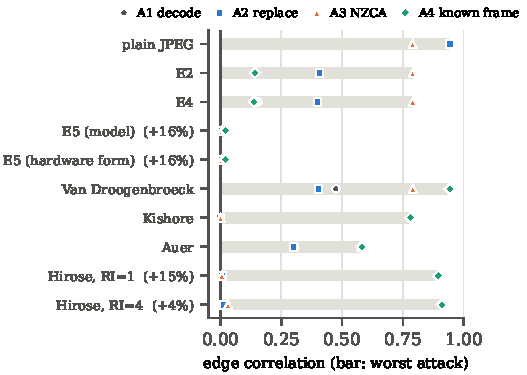
\includegraphics[width=\columnwidth]{figures/fig_bench.pdf}
\caption{SVE-Bench in one view: edge correlation of every scheme under each attack, pooled over \BenchSources{} sources; the bar ends at the worst attack. Byte cost over plain JPEG in brackets when above 2\,\%.}
\label{fig:bench}
\end{figure}
Leakage numbers from different papers are not comparable: each uses its own images, attack and metric. We therefore re-implemented four format-compliant schemes from their papers~\cite{vandroogenbroeck2002,kishore2015,auer2013,hirose2024}, with our keystream so that only the scheme differs, and scored them and ours under the same four attacks on \BenchFrames{} frames of \BenchSources{} sources (Table~\ref{tab:bench}, Fig.~\ref{fig:bench}):
\begin{itemize}
\item[A1] decoding the protected stream as is;
\item[A2] the replacement attack;
\item[A3] non-zero counting: a picture built from the number of non-zero coefficients per block, which no field encryption hides~\cite{hirose2024};
\item[A4] a known-plaintext attacker that knows one frame in clear, recovers from it the permutation and the keystream bits of that frame, and applies them to the following frames.
\end{itemize}
At its strongest attack every published scheme leaks between \BenchPubMin{} and \BenchPubMax. Those with fixed key material fall to the one known frame, among them Hirose et al.\ with a restart marker after every block (\BenchHiroseOneCross), although it costs about as many bytes as E5 ($+$\BenchHiroseOneBytes\,\%). E1--E4 sit at the non-zero-counting ceiling of plain JPEG (\BenchPlainNzca). E5, whose keystream and permutation change with every frame (Proposition~\ref{prop:perm}), stays at or below \BenchEfiveMax{} under every attack, in both its model and its hardware form; a test checks that the pictures an eavesdropper makes of the two forms are pixel-identical. The difference between E5 and Hirose et al.\ with one block per segment is not the mechanism, which is the same, but that our permutation is keyed per frame.

% generated by paper/make_assets.py from paper/data -- do not edit
\begin{table*}[t]
\caption{The metrics image-encryption papers report, for every scheme of Table~\ref{tab:bench} (no-key picture; same frames). PSNR and SSIM of the luma against the original; entropy of the luma histogram (8: flat); correlation of adjacent pixels; NPCR/UACI between the pictures under two keys one bit apart, and between two frames one pixel apart. They were designed for full-image ciphers: a format-compliant scheme keeps the stream decodable by design, so read them next to Table~\ref{tab:bench}.}
\label{tab:bench-metrics}
\centering\small
\resizebox{\textwidth}{!}{%
\begin{tabular}{lrrrccc}
\toprule
Scheme & PSNR (dB) & SSIM & Entropy & Corr. h / v / d & NPCR / UACI key (\%) & NPCR / UACI 1 px (\%) \\
\midrule
plain JPEG & 42.7 & 0.97 & 5.93 & 0.90 / 0.90 / 0.86 & -- / -- & 0.1 / 0.0 \\
\midrule
E1 & 24.9 & 0.59 & 6.03 & 0.87 / 0.86 / 0.80 & 70.4 / 4.7 & 32.4 / 1.9 \\
E2 & 11.0 & 0.29 & 5.09 & 0.85 / 0.87 / 0.82 & 86.8 / 46.1 & 32.2 / 11.3 \\
E3 & 11.1 & 0.28 & 5.10 & 0.84 / 0.88 / 0.81 & 87.3 / 48.5 & 32.7 / 11.5 \\
E4 & 10.2 & 0.28 & 4.97 & 0.82 / 0.86 / 0.79 & 86.6 / 48.2 & 32.4 / 11.9 \\
E5 (model) & 8.0 & 0.15 & 7.00 & 0.91 / 0.90 / 0.83 & 94.9 / 34.4 & 46.8 / 15.0 \\
E5 (hardware form) & 8.0 & 0.14 & 6.99 & 0.91 / 0.90 / 0.83 & 95.0 / 34.3 & 0.3 / 0.0 \\
\midrule
Van Droogenbroeck~\cite{vandroogenbroeck2002} & 24.5 & 0.57 & 6.05 & 0.86 / 0.85 / 0.79 & 71.4 / 5.3 & 33.1 / 2.1 \\
Kishore~\cite{kishore2015} & 7.4 & 0.18 & 6.05 & 0.89 / 0.88 / 0.84 & 88.7 / 40.0 & 14.6 / 1.2 \\
Auer~\cite{auer2013} & 16.9 & 0.40 & 6.24 & 0.63 / 0.61 / 0.49 & 84.6 / 21.7 & 75.9 / 17.7 \\
Hirose, RI\,=\,1~\cite{hirose2024} & 8.0 & 0.14 & 7.00 & 0.91 / 0.90 / 0.83 & 95.2 / 34.7 & 46.7 / 14.9 \\
Hirose, RI\,=\,4~\cite{hirose2024} & 7.6 & 0.18 & 6.93 & 0.96 / 0.92 / 0.89 & 94.1 / 37.1 & 45.7 / 16.3 \\
\bottomrule
\end{tabular}}
\end{table*}

\textit{The metrics of image-encryption papers.} Table~\ref{tab:bench-metrics} gives, for every scheme, the metrics that image-encryption papers report. They rank the schemes differently from Table~\ref{tab:bench}: a scheme that scrambles symbols without hiding positions can score well on PSNR, entropy and NPCR while leaking its outline, because these metrics measure how noisy the picture looks, not what an attacker can extract from it.

\subsection{Jigsaw solvers and a chosen-plaintext attack}
\begin{figure}[t]
\centering
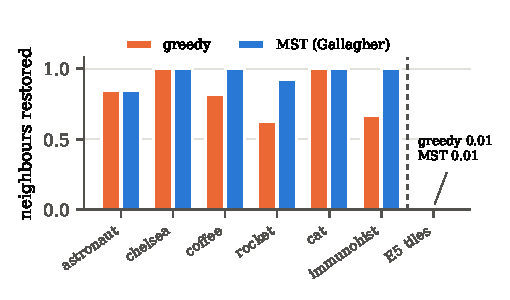
\includegraphics[width=\columnwidth]{figures/fig_jigsaw.pdf}
\caption{Neighbour pairs restored by the greedy and the minimum-spanning-tree solver on shuffled \emph{unencrypted} tiles of standard test photos (left) and on E5 tiles averaged over all sources (right).}
\label{fig:jigsaw}
\end{figure}
A permutation of blocks invites a puzzle solver. Our greedy region-growing solver in the style of~\cite{pomeranz2011} restores most neighbour relations on unencrypted shuffled tiles. On E5 replacement-attack tiles it places at most \JigsawNeighboursMax\,\% of neighbour pairs correctly, and the solved picture has no outline (Table~\ref{tab:leakage}). The structure is not destroyed, only hidden: an oracle that knew the permutation would recover edge correlations of \JigsawOracleMin--\JigsawOracleMax. A minimum-spanning-tree solver with Mahalanobis gradient compatibility~\cite{gallagher2012}, which restores at least \GateMstMin{} of the neighbours on unencrypted tiles of \GatePhotos{} photos (greedy: \GateGreedyMin), is also at chance on E5 (at most \MstNbMax\,\% on \MstSources{} sources, Fig.~\ref{fig:jigsaw}). The solvers fail because E5 also encrypts signs and amplitudes, so the borders of neighbouring tiles no longer match.

A chosen-plaintext attack~\cite{li2025shuffle} fails too: the attacker films a designed pattern whose per-block non-zero counts reveal the permutation. The permutation comes from the frame nonce, so on all \CpaSources{} sources one frame's exact permutation places at most \CpaPlacedEfive\,\% of the next frame's \CpaTiles{} tiles (chance) and leaves edge correlation $\le$\CpaEdgeEfive, where a key-only shuffle would give \CpaEdgeKeyMin--\CpaEdgeKeyMax.

\subsection{Sign-bit recovery by optimization}
% generated by paper/make_assets.py from paper/data -- do not edit
\begin{table}[t]
\caption{Sign-bit recovery attack of Lin et al.~\cite{lin2024} (LP relaxation, luma, 29 frames of 9 source sets). Top: their own setting on plain JPEG, where only the first $U$ AC signs per block are unknown (check of our implementation). Bottom: our levels, attacked from the ciphertext alone. Signs: share of unknown AC signs recovered, weighted by magnitude (chance 50\,\%). Edge: edge correlation with the original; last column: the replacement attack for comparison.}
\label{tab:signrec}
\centering\small
\resizebox{\columnwidth}{!}{%
\begin{tabular}{lrrrrr}
\toprule
Setting & Frames & Signs & SSIM & Edge & Repl.\ edge \\
\midrule
Lin et al.'s setting, $U{=}3$ & 29 & 93\,\% & 0.92 & 0.96 & -- \\
Lin et al.'s setting, $U{=}6$ & 29 & 88\,\% & 0.87 & 0.92 & -- \\
\midrule
E1 & 29 & 59\,\% & 0.45 & 0.41 & 0.33 \\
E2 & 29 & 49\,\% & 0.20 & 0.35 & 0.32 \\
E3 & 29 & -- & 0.21 & 0.36 & 0.31 \\
E4 & 29 & -- & 0.16 & 0.30 & 0.31 \\
\bottomrule
\end{tabular}}
\end{table}

The linear program of Lin et al.~\cite{lin2024} treats the unknown signs as relaxed variables and minimizes the total variation of the picture subject to the known magnitudes and the pixel range. In their setting, where only the first three or six AC signs of a block are unknown, it recovers \SrLinSignsMin--\SrLinSignsMax\,\% of the signs. On our levels it recovers \SrEoneSigns\,\% of E1's signs (\SrEoneSignsMin--\SrEoneSignsMax\,\% per frame), where every AC sign is hidden, and \SrEtwoSigns\,\% of E2's (chance 50\,\%) on \SrFrames{} frames of \SrSources{} source sets. It still sharpens E1's keyless picture (edge \SrEoneEdge{} against \SrEoneReplEdge{} for the replacement attack) and E2's and E3's by a few hundredths (Table~\ref{tab:signrec}): E1--E4 leak outlines however the hidden values are guessed.

\subsection{Learned attackers}
% generated by paper/make_assets.py from paper/data -- do not edit
\begin{table}[t]
\caption{U-Net reconstruction, SSIM / edge corr.\ on unseen test clips. P1: Trailer A$\rightarrow$B, P2: Talk A$\rightarrow$B, P3: Sintel$\rightarrow$Tears of Steel, P4: three clips$\rightarrow$three others. Repl.: replacement attack, P4 test set.}
\label{tab:learned}
\centering\small\setlength{\tabcolsep}{3pt}
\resizebox{\columnwidth}{!}{%
\begin{tabular}{llcccc}
\toprule
Mode & Repl. & P1 & P2 & P3 & P4 \\
\midrule
E1 & 0.55 / 0.40 & 0.72 / 0.53 & 0.70 / 0.66 & 0.55 / 0.42 & 0.79 / 0.69 \\
E2 & 0.17 / 0.40 & 0.42 / 0.33 & 0.27 / 0.34 & 0.13 / 0.32 & 0.34 / 0.40 \\
E4 & 0.18 / 0.39 & 0.43 / 0.34 & 0.28 / 0.32 & 0.12 / 0.26 & 0.35 / 0.40 \\
E5 & 0.14 / 0.00 & 0.34 / -0.02 & 0.26 / 0.02 & 0.22 / 0.00 & 0.36 / 0.04 \\
\bottomrule
\end{tabular}}
\end{table}

% generated by paper/make_assets.py from paper/data -- do not edit
\begin{table}[t]
\caption{Learned attackers with controls, SSIM/edge correlation on unseen test sources. R: replacement attack; N: U-Net. P3: Sintel$\rightarrow$Tears of Steel; P4: four sources$\rightarrow$three others; P5: public corpus with an adversarial loss$\rightarrow$the Sintel trailer and the private clips. Controls use no ciphertext: the median training frame, recoloured with the frame statistics the E5 stream reveals or with the true ones.}
\label{tab:learned_ext}
\centering\small\setlength{\tabcolsep}{2.5pt}
\resizebox{\columnwidth}{!}{%
\begin{tabular}{lcccccc}
\toprule
 & \multicolumn{2}{c}{P3} & \multicolumn{2}{c}{P4} & \multicolumn{2}{c}{P5} \\
Mode & R & N & R & N & R & N \\
\midrule
E1 & 0.45/0.36 & 0.55/0.41 & 0.57/0.40 & 0.79/0.69 & 0.61/0.47 & 0.83/0.74 \\
E2 & 0.18/0.36 & 0.14/0.31 & 0.21/0.39 & 0.37/0.43 & 0.20/0.41 & 0.30/0.40 \\
E4 & 0.19/0.35 & 0.13/0.30 & 0.22/0.38 & 0.36/0.37 & 0.21/0.40 & 0.31/0.41 \\
E5 & 0.14/0.00 & 0.22/0.00 & 0.18/0.01 & 0.34/0.03 & 0.17/0.01 & 0.26/-0.01 \\
\midrule
No stream (median frame) &  & 0.21/0.04 &  & 0.25/0.00 &  & 0.28/0.06 \\
+ stats the stream reveals &  & 0.22/0.04 &  & 0.26/0.00 &  & 0.26/0.06 \\
+ true frame stats (oracle) &  & 0.23/0.04 &  & 0.36/0.04 &  & 0.36/0.08 \\
\bottomrule
\end{tabular}}
\end{table}

\begin{figure*}[t]
\centering
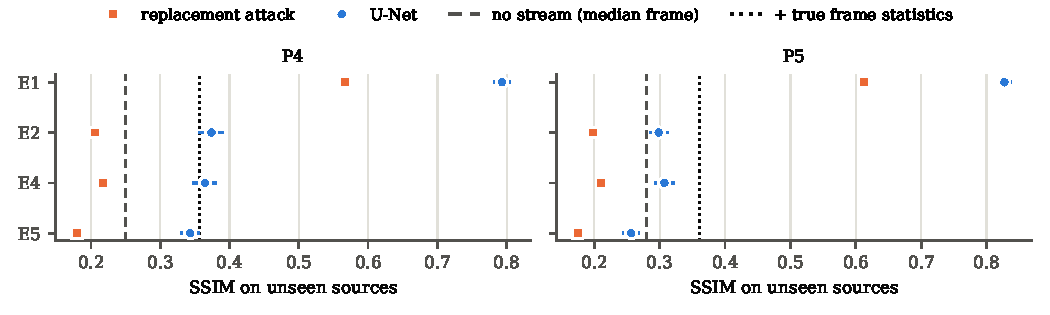
\includegraphics[width=0.85\textwidth]{figures/fig_learned.pdf}
\caption{SSIM of the learned attackers (U-Net, with 95\,\% interval) and of the replacement attack on unseen sources, per level. Dashed: the median training frame, which uses no ciphertext; dotted: the same frame recoloured with each test frame's true colour statistics. P4: four sources to three others; P5: trained on public films with an adversarial loss, tested on six other sources.}
\label{fig:learned}
\end{figure*}
We trained a U-Net~\cite{unet} to map the two keyless pictures (decoded and replacement attack) to the original and always tested it on clips it had not seen (Table~\ref{tab:learned}). P1 and P2 train on \LearnTrain{} frames of one clip, P3 uses only the open films, and P4 trains a wider network for \LearnBigEpochs{} epochs on \LearnBigTrain{} frames of \LearnBigTrainSrc{} sources and tests on \LearnBigTest{} frames of \LearnBigTestSrc{} others. The network defeats sign-only encryption: under E1 it reaches an edge correlation of \LearnEoneEdge{} and SSIM \LearnEoneSsim{} (replacement attack: \ReplEoneEdge{}), so E1 is no protection against a trained attacker. Under E2 and E4 it adds little to the outline that replacement already reveals (edge correlation \LearnEtwoFourEdgeMin--\LearnEtwoFourEdge{} against \ReplEtwoFourEdge) but raises SSIM to about \LearnEtwoFourSsimBig{} by learning brightness and colour.

\textit{Controls for frame-level statistics.} Table~\ref{tab:learned_ext} and Fig.~\ref{fig:learned} compare each learned attacker with three pictures that use no ciphertext: the median training frame, the same frame recoloured with the mean and spread of colour that the E5 stream itself reveals, and the same frame recoloured with the true statistics of each test frame. Under E5 the U-Net of P4 scores SSIM \LearnEfiveSsimBig{} [\LearnEfiveSsimLo, \LearnEfiveSsimHi], the oracle \CtrlTrueSsim{} [\CtrlTrueLo, \CtrlTrueHi]; the revealed-statistics control reaches \CtrlRevSsim. SSIM rewards flat pictures in smooth regions, so a flat picture of each frame's true mean colour already scores \FlatSsim; for this reason we read edge correlation, not SSIM, as the measure of recovered shape. Under E5 the network's edge correlation is \LearnEfiveEdgeBig{} against \CtrlTrueEdge{} for the oracle: what it learns from the stream is brightness and colour, not the shape of the scene.

\textit{An adversarial attacker on public data.} P5 trains the same U-Net for \PfiveEpochs{} epochs on \PfiveTrain{} frames of \PfiveCorpus{} with an additional least-squares adversarial loss (weight \PfiveAdv) from a PatchGAN discriminator~\cite{isola2017}, and is tested on \PfiveTest{} frames of \PfiveTestSrc{} sources it never saw. It is the strongest attacker on sign-only encryption (E1: edge correlation \PfiveEoneEdge, SSIM \PfiveEoneSsim), adds nothing to the outline that the replacement attack already shows under E2 and E4 (\PfiveEtwoFourEdge{} against \PfiveReplEtwoFourEdge), and recovers nothing under E5 (SSIM \PfiveEfiveSsim{} below the no-stream control of \PfiveCtrlSsim; edge correlation \PfiveEfiveEdge).

\subsection{Recognition}
\begin{figure}[t]
\centering
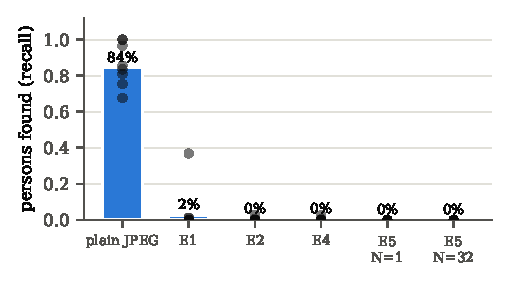
\includegraphics[width=\columnwidth]{figures/fig_recognition.pdf}
\caption{Share of the persons that a Faster R-CNN detector finds in the original frames and also finds, at the same place, in the eavesdropper's pictures (bars: pooled over \RecSources{} sources; dots: per source).}
\label{fig:recognition}
\end{figure}
% generated by paper/make_assets.py from paper/data -- do not edit
\begin{table}[t]
\caption{Person detection (Faster R-CNN, COCO) in the eavesdropper's pictures: recall (\%) of the persons found in the original frame, a detection in any attacker picture counting when it overlaps the original box (IoU $\ge$ 0.3). Sources with at least one person; 40 frames each (Kodak: 24 images).}
\label{tab:recognition}
\centering\small\setlength{\tabcolsep}{3pt}
\resizebox{\columnwidth}{!}{%
\begin{tabular}{lrrrrrrr}
\toprule
Source & Persons & Plain & E1 & E2 & E4 & E5/1 & E5/32 \\
\midrule
Trailer A & 69 & 75 & 0 & 0 & 0 & 0 & 0 \\
Trailer B & 63 & 81 & 0 & 0 & 0 & 0 & 0 \\
Talk A & 248 & 85 & 1 & 0 & 0 & 0 & 0 \\
Talk B & 38 & 100 & 37 & 3 & 3 & 0 & 0 \\
Phone A & 388 & 84 & 1 & 0 & 0 & 0 & 0 \\
Sintel & 34 & 68 & 0 & 0 & 0 & 0 & 0 \\
Tears of Steel & 29 & 97 & 0 & 0 & 0 & 0 & 0 \\
Kodak & 31 & 100 & 0 & 0 & 0 & 0 & 0 \\
\bottomrule
\end{tabular}}
\end{table}

Correlations measure whether a picture is in the right place; a person looking at the screen needs no such alignment. We therefore ran an off-the-shelf person detector, Faster R-CNN~\cite{ren2015} with a ResNet-50 FPN backbone trained on COCO, on the original and on every picture an eavesdropper can make, at a score threshold of 0.5, and counted an original person as found if an attacker picture has a detection overlapping it by an IoU of at least 0.3. Fig.~\ref{fig:recognition} and Table~\ref{tab:recognition} show the result over \RecPersons{} persons. On unprotected frames the detector finds \RecPlainMin--\RecPlainMax\,\% of them. Sign-only encryption already defeats it on most sources (\RecEonePooled\,\% pooled), but not on one talking-head clip (\RecEoneMax\,\%); under E2 and E4 it finds at most \RecEtwoFourMax\,\% on any source, and under E5 none. Detections anywhere in a frame, regardless of position, occur in at most \RecHitEtwoFiveMax\,\% of the frames with a person under E2--E5, about as often as false alarms on frames without one.

\subsection{Restart interval}\label{sec:restart}
% generated by paper/make_assets.py from paper/data -- do not edit
\begin{table}[t]
\caption{E5 with $N$ macroblocks per restart segment, mean over 5 sources at 320$\times$240. Overhead: bytes over the same E4 coefficients without markers. NZCA: correlation of the per-block count of non-zero coefficients with the original's block edge energy. Succ.: share of segments a beam-search solver chains to their true successor (chance in brackets).}
\label{tab:restart}
\centering\small\setlength{\tabcolsep}{3.5pt}
\resizebox{\columnwidth}{!}{%
\begin{tabular}{lccccc}
\toprule
$N$ & Segments & Perm.\ bits & Overhead (\%) & NZCA & Succ.\ (chance) \\
\midrule
E4 (no shuffle) & -- & -- & -- & 0.82 & -- \\
1 & 300 & 2041 & 15.2 & 0.01 & 0.02 (0.00) \\
2 & 150 & 873 & 7.5 & 0.01 & 0.03 (0.01) \\
4 & 75 & 363 & 3.8 & 0.02 & 0.04 (0.01) \\
8 & 38 & 149 & 1.9 & 0.02 & 0.03 (0.03) \\
10 & 30 & 108 & 1.5 & 0.02 & 0.08 (0.03) \\
32 & 10 & 22 & 0.5 & 0.04 & 0.27 (0.11) \\
\bottomrule
\end{tabular}}
\end{table}

E5 as specified costs \RiOverheadOneMin--\RiOverheadOneMax\,\% over the same E4 coefficients at 320$\times$240, as~\eqref{eq:e5cost} predicts: a two-byte marker per macroblock, padding and restarted DC prediction. $N$ macroblocks per segment reduce this to \RiOverheadFour\,\% at $N{=}4$ and \RiOverheadThirtyTwo\,\% at $N{=}32$ (Table~\ref{tab:restart}). Hirose et al.\ found that the non-zero counting attack reveals the scene unless the restart segments are permuted, and partly again when the restart interval is large~\cite{hirose2024}. Without the shuffle, our NZCA map correlates \RiNzcaEfourMin--\RiNzcaEfourMax{} with the original's block edge energy; with it, at most \RiNzcaEfiveMax{} for every $N$ we tried. At $N{=}32$, however, only \RiSegThirtyTwo{} segments remain, each an intact strip of 32 macroblocks, and a beam-search solver that chains segments by border continuity links \RiSuccThirtyTwoMin--\RiSuccThirtyTwoMax{} of them to their true successor on the real clips (chance \RiChanceThirtyTwo), against at most \RiSuccSmallMax{} for $N\le 8$. We keep $N{=}1$ and do not claim that longer intervals are safe.

\subsection{Standard metrics and key sensitivity}
% generated by paper/make_assets.py from paper/data -- do not edit
\begin{table}[t]
\caption{Standard image-encryption metrics, mean over 8 sources (5--6 frames each). Wrong key: the receiver's output with a key that differs in one bit, compared with the original (SSIM) and with the right decryption (NPCR/UACI, \%). 1-pixel: NPCR between two ciphertexts of frames that differ in one pixel, same key and nonce. Ideal values for a full-image cipher: NPCR 99.6, UACI 33.5, entropy 8, adjacent correlation 0.}
\label{tab:std}
\centering\small\setlength{\tabcolsep}{3pt}
\resizebox{\columnwidth}{!}{%
\begin{tabular}{lccccc}
\toprule
Level & Wrong-key SSIM & NPCR / UACI & 1-pixel NPCR & Entropy & Adj.\ corr. \\
\midrule
plain & -- & -- & -- & 5.88 & 0.93 \\
E1 & 0.58 & 70.3 / 4.9 & 33.8 & 6.02 & 0.89 \\
E2 & 0.27 & 89.8 / 46.3 & 35.5 & 5.40 & 0.92 \\
E3 & 0.25 & 87.8 / 42.9 & 33.3 & 5.25 & 0.91 \\
E4 & 0.24 & 88.8 / 47.5 & 34.5 & 5.14 & 0.91 \\
E5 & 0.13 & 95.8 / 35.8 & 46.8 & 7.07 & 0.88 \\
\bottomrule
\end{tabular}}
\end{table}

On all \StdSources{} sources (Table~\ref{tab:std}), key sensitivity holds: a one-bit key change makes E5 decryption differ in \StdNpcrEfiveMin--\StdNpcrEfiveMax\,\% of the pixels (SSIM $\le$\StdWrongSsimEfiveMax); in practice the receiver rejects such a frame because its tag fails. The other metrics assume a cipher that turns the image into noise: the 8$\times$8 block structure survives, so adjacent-pixel correlation stays at \StdCorrMin--\StdCorrMax{} and entropy rises only under E5 (\StdEntropyPlain{} to \StdEntropyEfive{} bits), and the 1-pixel NPCR (at most \StdPixelNpcrMax\,\%) measures diffusion, which a stream cipher with a fresh nonce per frame does not need: a one-pixel change of the plaintext under the same nonce never happens, because every frame has its own counter.

\subsection{Security summary}
Against goal G1, E1 is broken by a trained network and E2--E4 leak the outline under every attack we tried, however many bits they encrypt; E5 removed the outline under all of them, including known plaintext, chosen plaintext, two puzzle solvers, sign recovery and two trained networks, at a byte cost of \RiOverheadOneMin--\RiOverheadOneMax\,\%. What E5 leaks is the frame's colour statistics and its size; Section~\ref{sec:discussion} treats the latter.

% =====================================================================================================
\section{Protocol and Defence Evaluation}\label{sec:protocol}
\textit{Setup.} Sender, network channel, receiver and logger run as separate processes that talk over UDP, so the evaluation exercises the real wire format, fragmentation and timing. The sender encodes 320$\times$240 video at 10 frames/s with the golden model (the same bytes as the RTL), fragments every frame into datagrams of at most 1400 bytes and sends them; the channel can impose loss, delay, jitter and reordering and implements the attacker of Section~\ref{sec:threat}. All runs used a 4-core cloud virtual machine; the same scripts run against the board (Section~\ref{sec:board}).

\textit{Active attacks.} The full scenario applies \NumAttacks{} attacks for six seconds each, 25\,s apart: bit flips in the scan, a mode downgrade in the header, splicing of two frames, injection of a forged frame, replay, delay, dropping, a junk flood, and dropping, forging and replaying feedback. Table~\ref{tab:attacks} gives the result over \SuiteRuns{} runs. Every attack was mitigated in every run, on average \TtmMean{}\,$\pm$\,\TtmSd{}\,s after it began, with \SuiteFalse{} false alarms in calm windows and a median frame latency of \SuiteLatency\,ms. The slowest case, dropped feedback, is caught only by the dead-man rule, after about \FbDropTtm\,s: the 3\,s timeout plus part of a decision window. With a trailer, a talking-head clip or Tears of Steel as the video source instead of the synthetic scene, all attacks were again mitigated (\RealTrailerMit{}, \RealTalkMit{} and \RealOpenMit{}; means \RealTrailerTtm{}, \RealTalkTtm{} and \RealOpenTtm{}\,s, one run each) without false alarms.

% generated by paper/make_assets.py from paper/data -- do not edit
\begin{table}[t]
\caption{Reaction to each active attack (full suite, threshold policy, 3 runs; mean\,$\pm$\,s.d. in seconds). ``First rejection'' is when the receiver first discards a frame; ``mitigated'' is when the sender has raised protection or rekeyed.}
\label{tab:attacks}
\centering\small\setlength{\tabcolsep}{4pt}
\resizebox{\columnwidth}{!}{%
\begin{tabular}{lccc}
\toprule
Attack & Mitigated & First rejection & Mitigated after \\
\midrule
bit flips in the scan & 3/3 & 0.09\,$\pm$\,0.03 & 0.41\,$\pm$\,0.02 \\
mode downgrade in header & 3/3 & 0.06\,$\pm$\,0.02 & 0.44\,$\pm$\,0.02 \\
splice of two frames & 3/3 & 0.13\,$\pm$\,0.00 & 0.46\,$\pm$\,0.01 \\
forged frame injection & 3/3 & 0.14\,$\pm$\,0.06 & 0.44\,$\pm$\,0.03 \\
frame replay & 3/3 & 0.07\,$\pm$\,0.05 & 0.46\,$\pm$\,0.03 \\
frame delay & 3/3 & 4.13\,$\pm$\,0.04 & 1.46\,$\pm$\,0.03 \\
frame dropping & 3/3 & -- & 1.46\,$\pm$\,0.03 \\
junk flood & 3/3 & -- & 0.49\,$\pm$\,0.04 \\
feedback dropping & 3/3 & -- & 3.47\,$\pm$\,0.05 \\
forged feedback & 3/3 & -- & 0.46\,$\pm$\,0.04 \\
feedback replay & 3/3 & -- & 0.44\,$\pm$\,0.01 \\
\bottomrule
\end{tabular}}
\end{table}


\begin{figure*}[t]
\centering
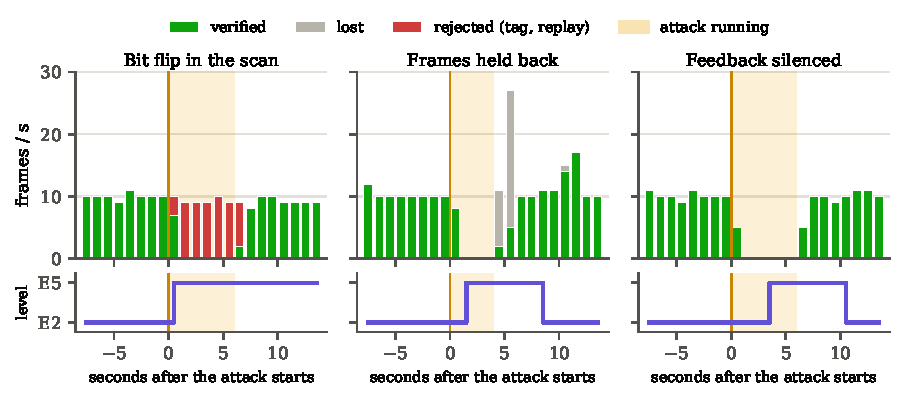
\includegraphics[width=0.92\textwidth]{figures/fig_case_evidence.pdf}
\caption{Three attacks as the sender sees them (one full-suite run): frames per second from the receiver's authenticated heartbeats, and the protection level. A bit flip fails the tag at once; held-back frames produce no rejection while the attack lasts and return as a gap of lost frames; silenced feedback leaves the receiver's video intact but blinds the sender until the dead-man rule fires.}
\label{fig:caseevidence}
\end{figure*}

\textit{The evidence decides the reaction time.} The attacks of Table~\ref{tab:attacks} are all mitigated, but Fig.~\ref{fig:caseevidence} shows that they leave three different kinds of evidence, and the evidence, not the harm, sets how fast the defence can react. A bit flip is the easy case: the receiver rejects the first tampered frame after \CaseBitflipFirstRej\,s on average over \CaseRuns{} runs and the sender reaches E5 after \CaseBitflipAware\,s. Holding frames back produces no rejection while it lasts, because nothing arrives at all. When the next frame gets through, the receiver counts the gap as lost frames; the held frames, released after the \CaseDelayDuration\,s attack, still carry valid tags but are older than frames already shown, so they are discarded as late (\CaseDelayRejected{} per run, the first \CaseDelayFirstRej\,s after the attack began), the verdict our replay window gives to benign reordering. The defence therefore never sees a delay: it reacts after \CaseDelayAware\,s to video that stops while heartbeats still arrive, which it treats as jamming. Silencing the feedback path is the mirror image. The receiver sees perfect video and rejects \CaseFbdropRejected{} frames, yet the sender, which learns about the link only through authenticated heartbeats, goes blind, and only the dead-man rule escalates, after \CaseFbdropAware\,s. The stream stays at its floor level longest during this attack, which gives it the highest leakage of all attacks while active (\CaseFbdropLeak, the mean edge correlation of the active level). Integrity attacks are caught at the first frame; attacks by absence can only be caught by a timeout, so their reaction time is a design parameter, and shortening it trades against false alarms on a slow network.

\textit{Benign impairments.} A second scenario applies only network problems: rising packet loss up to 6\,\%, delay up to 120\,ms with jitter, and 5\,\% reordering. Over \BenignRuns{} runs the defence raised no false alarm (\BenignFalse{} windows); median latency was \BenignLatency\,ms and the 95th percentile \BenignPninetyfive\,ms. This needed loss to be judged over three windows and late frames to be told apart from replays.

\begin{figure}[t]
\centering
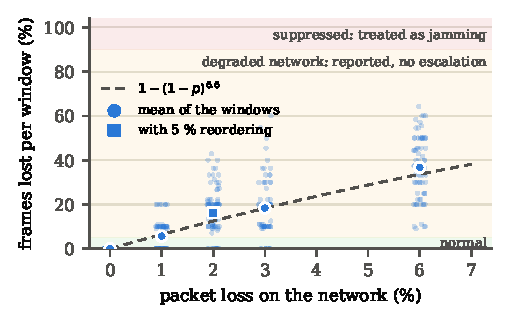
\includegraphics[width=\columnwidth]{figures/fig_case_loss.pdf}
\caption{Frame loss against packet loss in the benign scenario (\BenignRuns{} runs; small dots: one-second windows, large: means). The dashed curve is~\eqref{eq:fragloss}, fitted to the points without reordering. The shading is the policy's classification of frame loss.}
\label{fig:caseloss}
\end{figure}
\textit{A third of the frames lost, and no alarm.} A frame of $n$ fragments is lost when any fragment is, so with independent packet loss $p$
\begin{equation}
P_{\mathrm{frame}} = 1 - (1 - p)^n \approx n p \quad (np \ll 1).
\label{eq:fragloss}
\end{equation}
Fig.~\ref{fig:caseloss} shows how badly a lossy network treats a fragmented video stream: at \CaseSixPct\,\% packet loss the receiver lost \CaseSixFrameLoss\,\% of the frames, \CaseAmplification{} times the packet loss, and the points without reordering follow~\eqref{eq:fragloss} with $n \approx \CaseFragments$ fragments per frame. Even so, the defence did not escalate once, because loss between 5 and 90\,\% is reported as a degraded network; the highest threat score~\eqref{eq:threat} of any benign window was \CaseBenignMaxThreat, half the level at which Table~\ref{tab:attacks} counts the sender as aware. The same rule is a limitation: jamming that lets more than a tenth of the frames through is indistinguishable from a bad network. Forward error correction across fragments would lower the curve, at a bitrate cost.

\textit{Threshold rule against bandit.} The learning scenario repeats a bit-flip and a replay attack five times each, separated by calm periods. We ran both policies with \Seeds{} paired seeds (Table~\ref{tab:policies}, Fig.~\ref{fig:policies}). The result is a consistent trade-off rather than a winner. The bandit encrypted fewer bits in every seed (\PolCostB{} against \PolCostT{} of the payload, \PolCostSave\,\% less), but it reacted later (\PolTtmB{} against \PolTtmT\,s) and leaked more while attacks were active (\PolLeakB{} against almost zero), again in every seed. Neither policy raised a false alarm (\PolFalse{}). The reason is the loss~\eqref{eq:loss}: the bandit pays for encrypted bits in every calm window and for leakage only in the windows after an attack is visible, so it learns to sit lower and climb when evidence appears. We keep the threshold rule as the default; the bandit suits links where bandwidth matters more than the first second of an attack.

% generated by paper/make_assets.py from paper/data -- do not edit
\begin{table}[t]
\caption{Threshold rule vs.\ $\varepsilon$-greedy bandit on the learning scenario, 10 seeds each (mean\,$\pm$\,s.d.). The last column counts the seeds in which the bandit was better (lower) than the threshold rule with the same seed.}
\label{tab:policies}
\centering\small\setlength{\tabcolsep}{4pt}
\resizebox{\columnwidth}{!}{%
\begin{tabular}{lccc}
\toprule
Metric & Threshold & Bandit & Bandit better \\
\midrule
Mitigation (s) & 0.46\,$\pm$\,0.02 & 1.34\,$\pm$\,0.03 & 0/10 \\
Leakage under attack & 0.000\,$\pm$\,0.001 & 0.054\,$\pm$\,0.004 & 0/10 \\
Encrypted share & 0.188\,$\pm$\,0.001 & 0.162\,$\pm$\,0.001 & 10/10 \\
Encrypted share, calm & 0.135\,$\pm$\,0.000 & 0.138\,$\pm$\,0.001 & 0/10 \\
\bottomrule
\end{tabular}}
\end{table}

\begin{figure}[t]
\centering
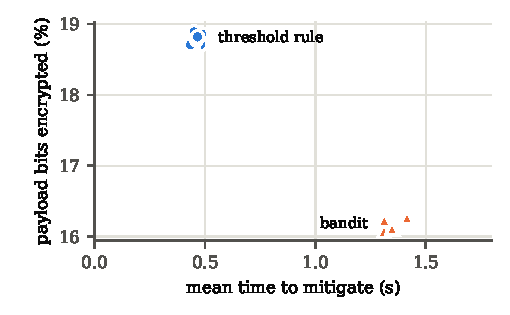
\includegraphics[width=\columnwidth]{figures/fig_policies.pdf}
\caption{Encrypted share of the payload against mean time to mitigate, one point per seed and policy (\Seeds{} paired seeds).}
\label{fig:policies}
\end{figure}

\textit{Cost relative to software.} On the simulation host, our Python model needs \PyPlainMs\,ms to encode a 640$\times$480 frame and \PySelEtwoMs\,ms including E2 selective encryption, whereas libjpeg-turbo takes \TurboMs\,ms and full-stream AES-GCM about \AesGcmMs\,ms. A desktop processor is the wrong baseline; what matters is the SoC's ARM core, which has no AES instructions (Section~\ref{sec:board}).

% =====================================================================================================
\section{Further Experiments}\label{sec:further}
\subsection{Bitrate regulation}
\begin{figure}[t]
\centering
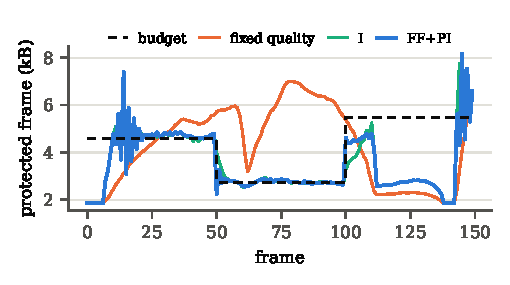
\includegraphics[width=\columnwidth]{figures/fig_rate_control.pdf}
\caption{Bitrate regulation on the Sintel trailer: protected frame size under a budget that follows the link (100\,\%, 60\,\%, 120\,\% of the clip's median), with fixed quality, integral control and feed-forward plus PI.}
\label{fig:rc}
\end{figure}
A sender on a shared link must follow the available bandwidth $B_k$. Treating the quality factor like the voltage of a motor drive, we compared fixed quality, bang-bang, integral, PI and feed-forward plus PI control (Fig.~\ref{fig:rc}). JPEG maps quality $q$ to the scale of the quantization tables as $5000/q$ below 50 and $200 - 2q$ above, so one quality step changes the bytes about four times more at low quality than at high quality; the controllers therefore act on $u = \ln(\text{scale})$, in which the plant is nearly linear, $\ln S_k \approx a - g\,u_k$, and on the logarithmic error
\begin{equation}
\varepsilon_k = \ln (B_k / S_k),
\label{eq:rcerr}
\end{equation}
which is symmetric (twice too big counts as much as half too small). The PI law in velocity form, with a slew limit $|\Delta u| \le \Delta_{\max}$, is
\begin{equation}
\begin{aligned}
\Delta u_k &= K_P (\varepsilon_k - \varepsilon_{k-1}) + K_I \varepsilon_k,\\
u_{k+1} &= u_k - \operatorname{clip}(\Delta u_k, \pm\Delta_{\max}),
\end{aligned}
\label{eq:pi}
\end{equation}
and the feed-forward term jumps by $\Delta u = -\ln(B_{k}/B_{k-1})/\hat g$ when the budget changes, with $\hat g$ estimated online by recursive least squares while the input is excited. After settling, fixed quality misses the budget by \RcFixedErrMin--\RcFixedErrMax\,\% on \RcClips{} real clips, integral control by \RcIErrMin--\RcIErrMax\,\% and feed-forward plus PI by \RcFfpiErrMin--\RcFfpiErrMax\,\%, which settles within \RcFfpiSettleMax{} frames of a bandwidth drop (\RcSynFfpiErr\,\% on the synthetic scene). Scene cuts are disturbances that no causal controller anticipates. A controller tuned in the quality domain oscillated at low quality on one clip; acting on $u$ keeps the loop gain nearly constant over the whole range.

\subsection{Change-driven coding}
\begin{figure}[t]
\centering
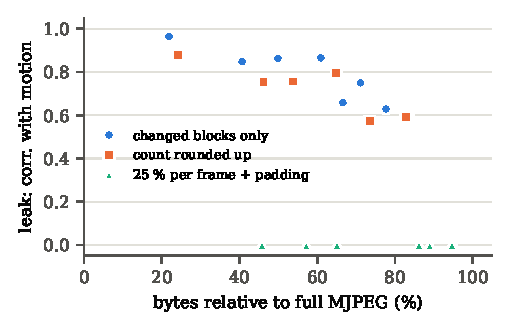
\includegraphics[width=\columnwidth]{figures/fig_change_driven.pdf}
\caption{Change-driven coding: bytes against the leak of motion (the larger correlation of the per-frame block count or frame size with the true motion) for three policies, one point per source. Only coding a constant share of blocks and padding every frame hides motion.}
\label{fig:change}
\end{figure}
Coding only the 16$\times$16 blocks that changed, as a retina does, needs \CdBytesFixed\,\% of the bytes on the fixed camera but \CdBytesMin--\CdBytesMax\,\% on the real clips, and the number of coded blocks tracks motion (correlation \CdCountFixed{} and \CdCountMin--\CdCountMax) even when the change map is hidden (Fig.~\ref{fig:change}). Coding a constant 25\,\% of the blocks per frame, refreshing the oldest unchanged ones, and padding every frame hides both, at \CdPadFixed\,\% of the bytes and SSIM \CdPadSsimFixed{} on the fixed camera, but SSIM falls to \CdPadSsimMin--\CdPadSsimMax{} on edited clips.

\subsection{Keyed block transforms}
Independent keyed flips per block defeat jigsaw solvers for block-scrambling ciphers. For the DCT, a flip is a pattern of sign changes, which E5 already encrypts: on \BtSources{} sources the jigsaw solver stays at chance (at most \BtNbMax\,\% neighbours) with or without keyed flips, and even with every tile position given, SSIM changes by at most \BtSsimDelta. E5's protection therefore rests on the block positions; an attacker who knew them would reach SSIM \BtOracleMin--\BtOracleMax{} on the real clips (\BtOracleFixed{} on the synthetic scene).

% =====================================================================================================
\section{Discussion and Limitations}\label{sec:discussion}
\begin{figure}[t]
\centering
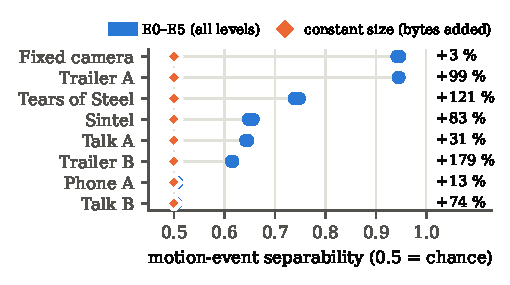
\includegraphics[width=\columnwidth]{figures/fig_size_channel.pdf}
\caption{Motion events detected from frame sizes alone, for every protection level (bar: E0--E5 range) and with every frame padded to a constant size (diamond; bytes added on the right). Fixed camera: synthetic scene; the others are the real clips.}
\label{fig:size}
\end{figure}
% generated by paper/make_assets.py from paper/data -- do not edit
\begin{table}[t]
\caption{Which of 7 videos is playing, identified from $W$ consecutive encrypted frame sizes (after~\cite{schuster2017}), in \% of 300 queries; chance 14\,\%. At 10 frames/s, $W{=}10$ is one second. Bytes: cost over the E2 stream.}
\label{tab:fingerprint}
\centering\small
\resizebox{\columnwidth}{!}{%
\begin{tabular}{lrrrrr}
\toprule
Stream & Bytes & $W{=}5$ & $W{=}10$ & $W{=}30$ & $W{=}100$ \\
\midrule
E1--E4 & +0\,\% & 76 & 98 & 100 & 100 \\
E5 & +12\,\% & 69 & 99 & 100 & 100 \\
pad to 1\,KB & +6\,\% & 21 & 40 & 85 & 97 \\
pad to running max. & +55\,\% & 18 & 23 & 31 & 46 \\
pad to 10\,s max. & +41\,\% & 18 & 31 & 52 & 95 \\
constant size & +81\,\% & 14 & 13 & 19 & 14 \\
\bottomrule
\end{tabular}}
\end{table}

\textit{What no level hides.} Encryption hides content, not length. Frame sizes reveal motion at every level alike (Fig.~\ref{fig:size}). They also identify a known video, as Schuster et al.\ showed for encrypted streaming~\cite{schuster2017}: an attacker who encodes candidate videos himself and correlates the size sequence picks the right one of \FpVideos{} videos from ten frame sizes \FpEtwoTen\,\% of the time under E1--E4 and \FpEfiveTen\,\% under E5 (chance \FpChance\,\%, Table~\ref{tab:fingerprint}). Padding to 1\,KB steps lowers that to \FpKbTen\,\% for $+$\FpKbCost\,\% bytes but not over 100 frames (\FpKbHundred\,\%), padding to the running maximum to \FpRunTen\,\% for $+$\FpRunCost\,\%, and only constant-size frames reach chance, at $+$\FpConstCost\,\% on these edited clips. Constant-size frames close the channel cheaply for a fixed camera ($+$\PadFixed\,\%) but cost up to $+$\PadFilmMax\,\% bytes on edited clips; padding to the largest frame so far gives a separability of \PadRunSep{} for $+$\PadRunCost\,\% on the fixed camera (\PadRunFilmSepMin--\PadRunFilmSepMax{} on the real clips), while bitrate regulation lets up to \RcPadOverMax\,\% of frames exceed a cap. A surveillance camera is the favourable case: its scene is fixed and padding is cheap.

\textit{Limitations.} Five limitations bound our claims. First, the board confirms correctness but not yet speed or power: the encoder is bit-exact on the PYNQ-Z2, but our frame rate there is set by a Python driver on the ARM, the fabric-only time and the power are not yet measured on the board, and the power figures come from simulated switching activity; whether DDR feeds the four-lane encoder its \RtlFourLanesInMBs\,MB/s of pixels is also open. Second, sign and amplitude encryption leak outlines by construction (Lemma~\ref{lem:format}), however many bits are encrypted; only a change of block positions removes them, at a bitrate cost. Third, frame sizes leak at every level, as above. Fourth, our attackers are greedy or trained on a few clips; stronger puzzle solvers or attackers trained on large video corpora may extract more from E5, and a trained network already undoes sign-only encryption (E1). Fifth, the master key is pre-shared; a key exchange such as X25519 on the ARM core at session start, as DTLS-SRTP does for SRTP~\cite{rfc3711}, would remove that assumption without touching the fabric. On the protocol side, the receiver cannot tell heavy benign loss from partial jamming, so only near-total suppression escalates, and the reaction time is bounded below by the one-second decision window.

\textit{Reproducibility and data.} Every number in this paper is produced by a script from stored results and inserted into the text by a generator, never typed; a test fails if a table in the manuscript differs from what the data produce. The open sources (the Blender Foundation films and the Kodak images) can be downloaded and rerun; the private clips are identified by SHA-256 hash and never shown, and frames of them are never stored as images. The golden model, the RTL, the testbenches, the Vivado and board scripts, the experiment scripts and the scripts that rerun all GPU and long-CPU experiments in one cloud session are available in our repository.

\textit{Lessons.} Three kinds of error recurred while building this system, and each changed how we work. Simulation-only success hid timing problems that only place and route exposed, so post-route numbers are now part of every hardware claim. Experiment scripts were wrong more often than the RTL: a set point that clips opening on black could not reach, an estimator that wound up when its input saturated, a controller tuned at one operating point and unstable at another, and a test source that stamped the wall-clock time into every frame. Each was found because a result looked implausible on new data, and each now has a regression test. Finally, two claims had to be withdrawn when stronger evidence arrived: the E5 edge correlation of the U-Net is above that of the plain prior once more data is used, which the frame-statistics control explains, and the cost of hiding frame sizes is small only for fixed cameras.

\textit{Ethics.} The clips with identifiable people are used only to measure what an eavesdropper could recover; no picture derived from them appears here, and none is stored.

% =====================================================================================================
\section{Conclusion}\label{sec:conclusion}
Encrypting coefficient signs and amplitudes with Ascon inside a JPEG encoder costs no cycles, provably keeps every protection level playable, and, combined with a per-frame tag over metadata and scan, turns a plain MJPEG stream into an authenticated one. Field encryption alone, however, leaves the outline of the scene to anyone who counts non-zero coefficients, and published format-compliant schemes also fall to one known frame because their key material does not change. A keyed permutation of macroblocks that is drawn anew for every frame removes the outline under every attack we could build, and with restart segments it fits in hardware without a frame buffer: the fabric codes and authenticates the segments, the processor only reorders them. Parallel lanes over the same segments raise throughput to \RtlFourLanesMpix\,Mpixel/s at 100\,MHz, and a closed feedback loop answers active network attacks within about a second in simulation. No level hides frame sizes, which identify a known video and reveal motion; constant-size frames close that channel at a cost that is small only for fixed cameras. Next are the fabric-only time and power on the board, a driver that keeps the ARM off the pixel path, size padding in hardware, a shared Ascon core across lanes, a 125\,MHz clock, key derivation with the standard's extendable-output function, and a key exchange at session start.


\section*{Acknowledgment}
We thank Dr.~Chetana~G for her guidance. \TODO{AI-assistance disclosure as required by IEEE (see paper/README.md): name the tools and what they were used for, e.g.\ code generation, test scaffolding and language editing.}

\bibliographystyle{IEEEtran}
\bibliography{refs}

\begin{IEEEbiographynophoto}{Aravind R}
\TODO{biography and photo (1 in $\times$ 1.25 in), as the IEEE Access template requires}
\end{IEEEbiographynophoto}
\begin{IEEEbiographynophoto}{Suhas V J}
\TODO{biography and photo}
\end{IEEEbiographynophoto}
\begin{IEEEbiographynophoto}{Rishab H R}
\TODO{biography and photo}
\end{IEEEbiographynophoto}
\begin{IEEEbiographynophoto}{Samarth B N}
\TODO{biography and photo}
\end{IEEEbiographynophoto}
\begin{IEEEbiographynophoto}{Vijaysurya B S}
\TODO{biography and photo}
\end{IEEEbiographynophoto}
\begin{IEEEbiographynophoto}{Chetana G}
\TODO{biography and photo}
\end{IEEEbiographynophoto}
\EOD
\end{document}
